\documentclass[11pt,a4paper]{article}
\usepackage[utf8]{inputenc}
\usepackage[margin=0.8in]{geometry}
\setlength{\headheight}{14pt}
\usepackage{graphicx}
\usepackage{amsmath,amssymb}
\usepackage{booktabs}
\usepackage{longtable}
\usepackage{array}
\usepackage{hyperref}
\usepackage{float}
\usepackage{caption}
\usepackage{subcaption}
\usepackage{fancyhdr}
\usepackage{titlesec}
\usepackage{xcolor}

% Custom Colors
\definecolor{primary}{RGB}{0, 51, 102}
\definecolor{secondary}{RGB}{70, 130, 180}

\hypersetup{
    colorlinks=true,
    linkcolor=primary,
    citecolor=primary,
    urlcolor=secondary
}

% Header and Footer setup
\pagestyle{fancy}
\fancyhf{}
\rhead{\textcolor{primary}{\textbf{EDC Laboratory --- Experiment 3}}}
\lhead{\textcolor{primary}{\textbf{EE25BTECH11056 \& EE25BTECH11049}}}
\rfoot{Page \thepage}

\titleformat{\section}{\large\bfseries\color{primary}}{\thesection.}{0.5em}{}
\titleformat{\subsection}{\normalfont\bfseries\color{secondary}}{\thesubsection}{0.5em}{}
\titleformat{\subsubsection}{\normalfont\bfseries}{\thesubsubsection}{0.5em}{}

\begin{document}

% Title Page / Header Block
\begin{center}
    {\LARGE \textbf{\color{primary} DEPARTMENT OF ELECTRICAL ENGINEERING}}\\[0.2cm]
    {\large \textbf{Electronic Devices \& Circuits Laboratory (EDC LAB)}}\\[0.4cm]
    \rule{\linewidth}{1pt}\\[0.3cm]
    {\Large \textbf{EXPERIMENT 3: Input (Transfer) \& Output (Drain) Characteristics of N-Channel Enhancement MOSFET (2N7000)}}\\[0.3cm]
    \rule{\linewidth}{1pt}\\[0.4cm]
    
    \begin{tabular}{ll}
      \textbf{Prepared By:} & \textbf{Suraj.N (EE25BTECH11056)} \\
                            & \textbf{Sai Krishna Bakki (EE25BTECH11049)} \\
        \textbf{Course:} & Electronic Devices \& Circuits Lab \\
        \textbf{Date:} & \today
    \end{tabular}
\end{center}

\vspace{0.3cm}

\section{Aim}
\begin{enumerate}
    \item To study and plot the \textbf{Output (Drain) Characteristics} ($I_D$ vs $V_{DS}$) of an N-Channel Enhancement-mode MOSFET (2N7000) for fixed values of Gate-Source voltage ($V_{GS} = 1.6\text{ V}, 1.8\text{ V}, 2.0\text{ V}$), and to determine the \textbf{drain (output) resistance ($r_d$)}.
    \item To study and plot the \textbf{Transfer (Input) Characteristics} ($I_D$ vs $V_{GS}$) of the MOSFET for fixed values of Drain-Source voltage ($V_{DS} = 5\text{ V}, 7\text{ V}, 9\text{ V}$), and to determine the \textbf{threshold voltage ($V_T$)} and \textbf{transconductance ($g_m$)}.
    \item To evaluate the small-signal \textbf{amplification factor ($\mu = g_m \cdot r_d$)} of the transistor.
\end{enumerate}

\section{Apparatus and Software Tools Required}
\begin{table}[H]
\centering
\caption{Equipment, Components, and Software Specifications}
\begin{tabular}{cllc}
\toprule
\textbf{S.No.} & \textbf{Component / Equipment} & \textbf{Specification} & \textbf{Quantity} \\
\midrule
1 & N-Channel MOSFET & 2N7000 (TO-92 package) & 1 \\
2 & Regulated DC Power Supplies & Variable $0\text{--}30\text{ V}$ Dual Output & 2 \\
3 & Digital Ammeter / Microammeter & $0\text{--}500\ \mu\text{A}$, $0\text{--}50\text{ mA}$ & 1 \\
4 & Digital Voltmeters & $0\text{--}30\text{ V}$ range & 2 \\
5 & Simulation Software & LTspice XVII & -- \\
\bottomrule
\end{tabular}
\end{table}

\section{Overall Theoretical Background}
A Metal-Oxide-Semiconductor Field-Effect Transistor (MOSFET) is a three-terminal (Gate, Drain, Source), voltage-controlled semiconductor device. The gate is electrically insulated from the semiconductor channel by a thin oxide layer ($SiO_2$), resulting in virtually zero DC gate current ($I_G \approx 0$).

In an N-channel enhancement-mode MOSFET:
\begin{itemize}
    \item \textbf{Cut-off Region ($V_{GS} < V_T$):} No conducting channel exists between drain and source. $I_D \approx 0$.
    \item \textbf{Triode / Ohmic Region ($V_{GS} \ge V_T$ and $V_{DS} < V_{GS} - V_T$):} An inversion channel is formed. $I_D$ increases almost linearly with $V_{DS}$, governed by:
    \begin{equation}
        I_D = k_n \left[ (V_{GS} - V_T) V_{DS} - \frac{1}{2} V_{DS}^2 \right]
    \end{equation}
    \item \textbf{Saturation Region ($V_{GS} \ge V_T$ and $V_{DS} \ge V_{GS} - V_T$):} The channel pinches off at the drain end. $I_D$ becomes independent of $V_{DS}$ (ignoring channel-length modulation) and follows the square law:
    \begin{equation}
        I_D = \frac{1}{2} k_n (V_{GS} - V_T)^2 (1 + \lambda V_{DS})
    \end{equation}
\end{itemize}

\clearpage

\section{Part A: Output (Drain) Characteristics ($I_D$ vs $V_{DS}$)}

\subsection{Theoretical Background}
The output characteristic is a plot of Drain Current ($I_D$) versus Drain-Source Voltage ($V_{DS}$) while holding the Gate-Source Voltage ($V_{GS}$) constant. 
\begin{itemize}
    \item At low $V_{DS}$ ($V_{DS} < V_{GS} - V_T$), the transistor acts as a voltage-variable resistor (Ohmic region).
    \item At $V_{DS} = V_{GS} - V_T$, pinch-off occurs. Beyond this point, the curve flattens into the saturation region.
    \item The reciprocal of the slope of the saturation curve defines the dynamic \textbf{drain (output) resistance ($r_d$)}:
    \begin{equation}
        r_d = \left. \frac{\Delta V_{DS}}{\Delta I_D} \right|_{V_{GS} = \text{const}}
    \end{equation}
\end{itemize}

\subsection{Circuit Schematic and LTspice Simulation Waveforms}
\begin{figure}[H]
    \centering
    
\includegraphics[width=0.55\textwidth]{../SIMULATIONS/Output/schematic.png}
    \caption{LTspice Circuit Schematic for Part A (Output Characteristics).}
    \label{fig:part_a_schematic}
\end{figure}

\begin{figure}[H]
    \centering
    \begin{subfigure}[b]{0.48\textwidth}
        \centering
        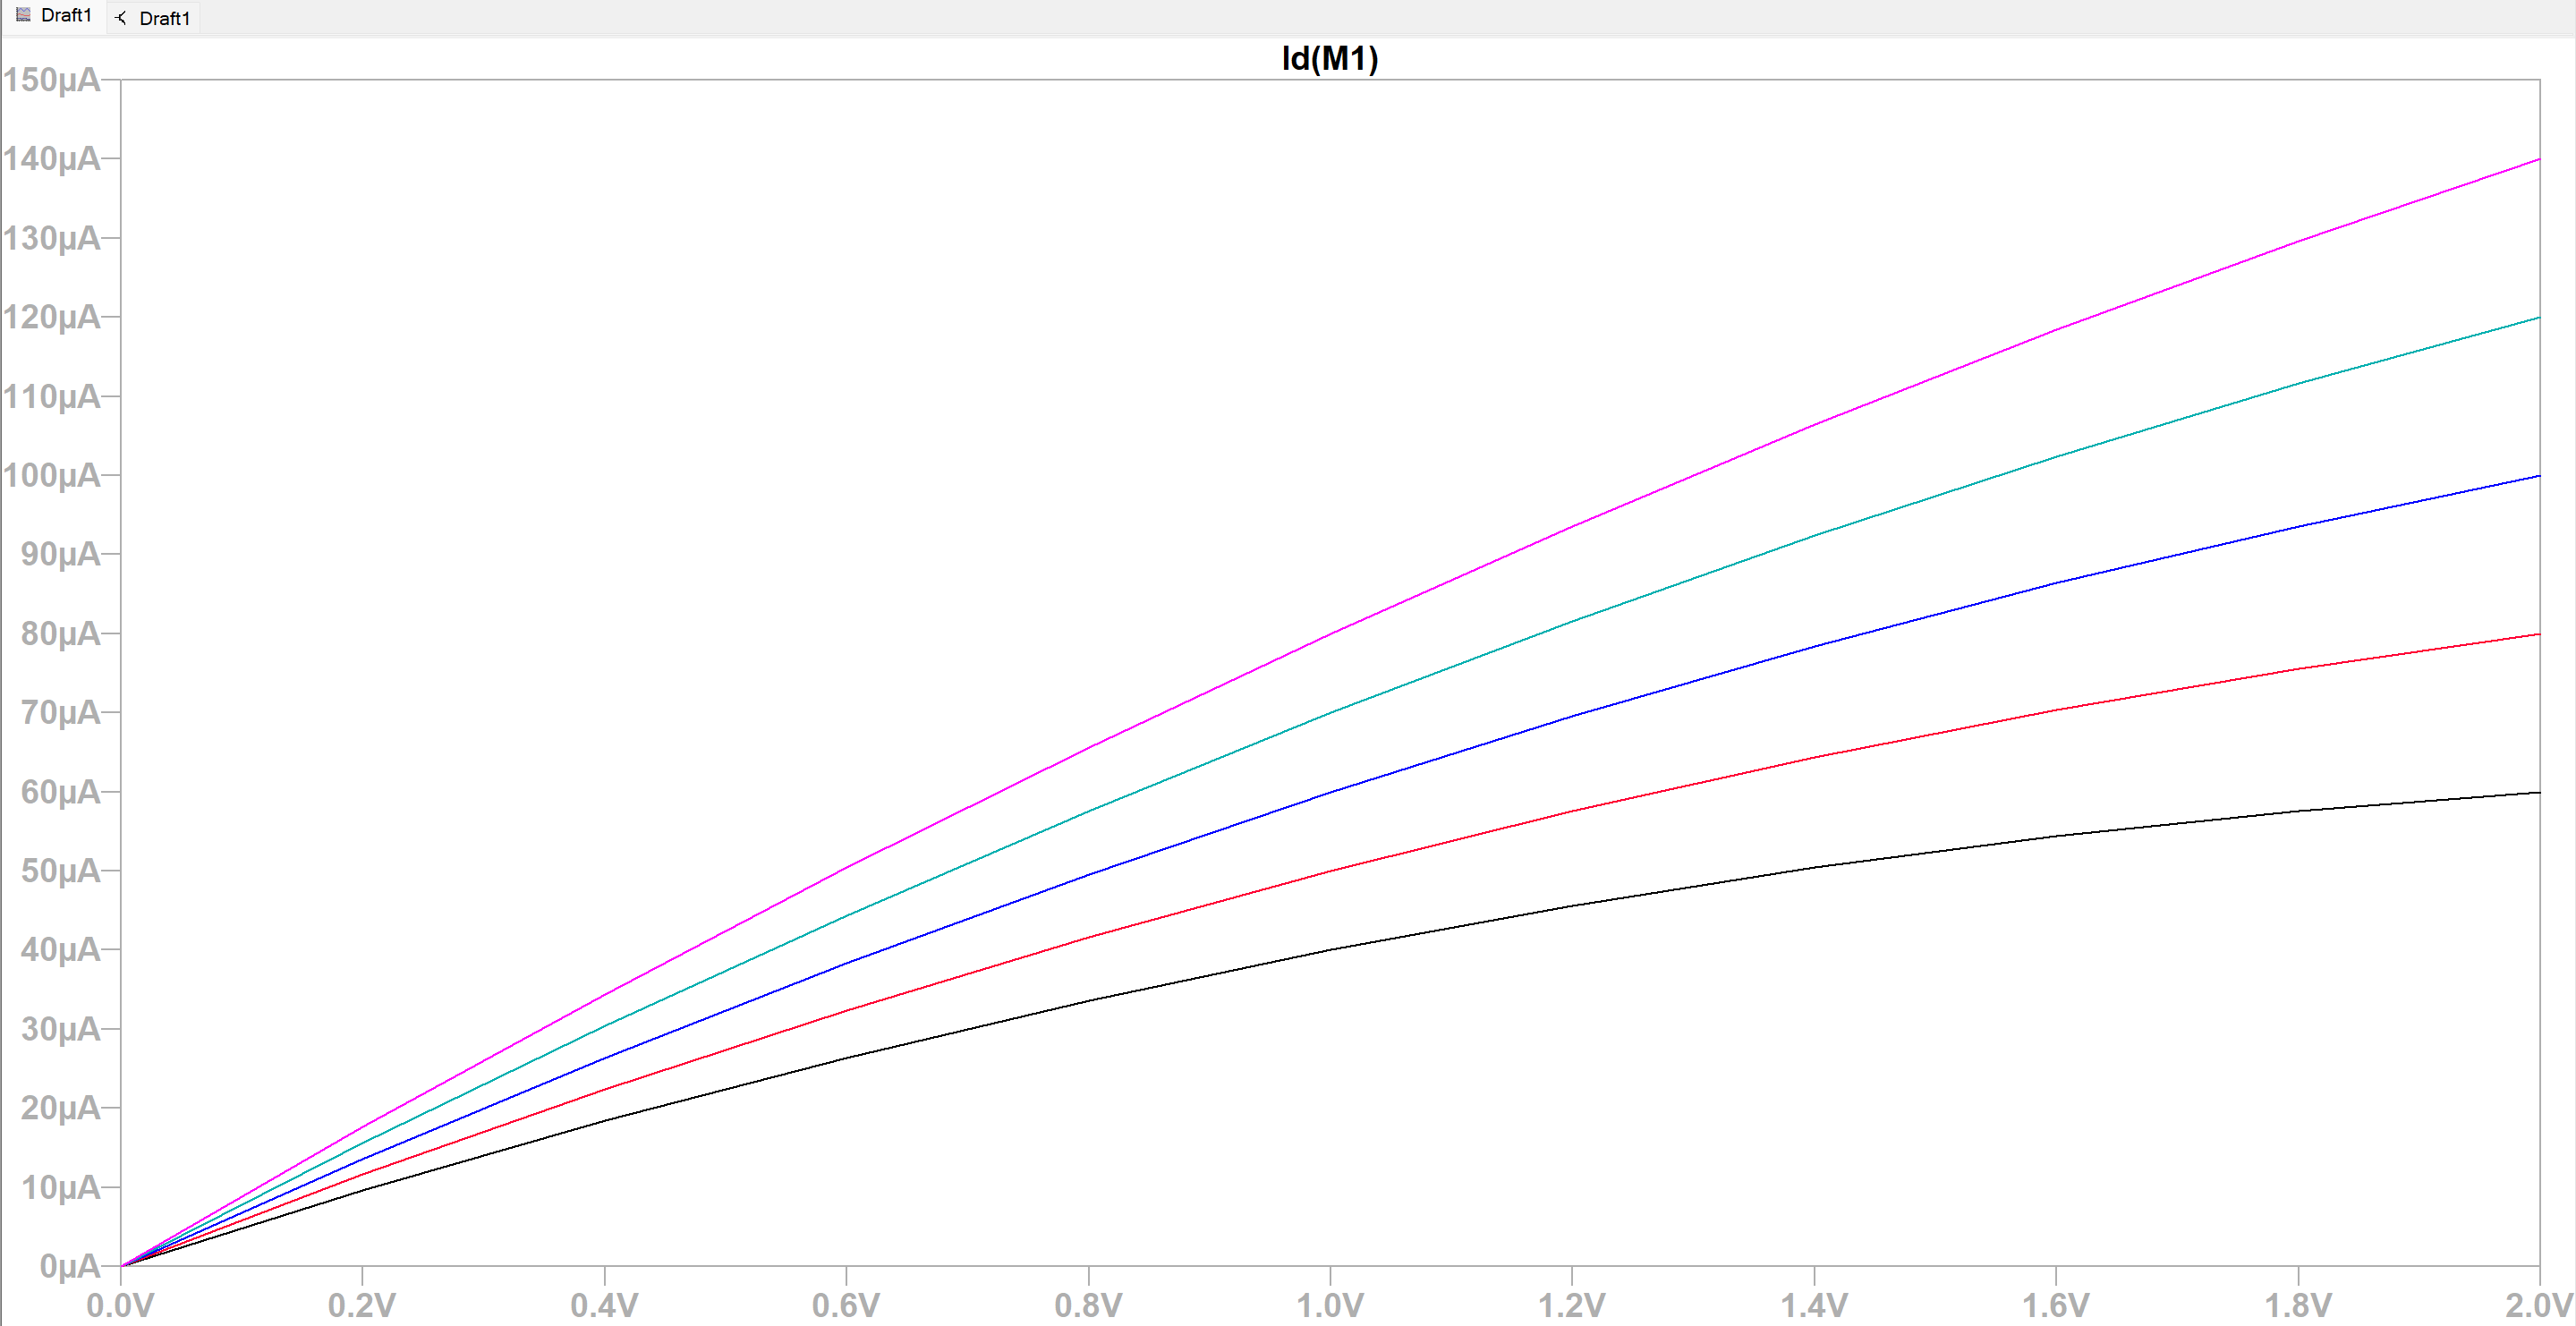
\includegraphics[width=\textwidth]{../SIMULATIONS/Output/output_(0-2V).png}
        \caption{Low $V_{DS}$ Sweep ($0\text{--}2\text{ V}$, Triode Region)}
    \end{subfigure}
    \hfill
    \begin{subfigure}[b]{0.48\textwidth}
        \centering
        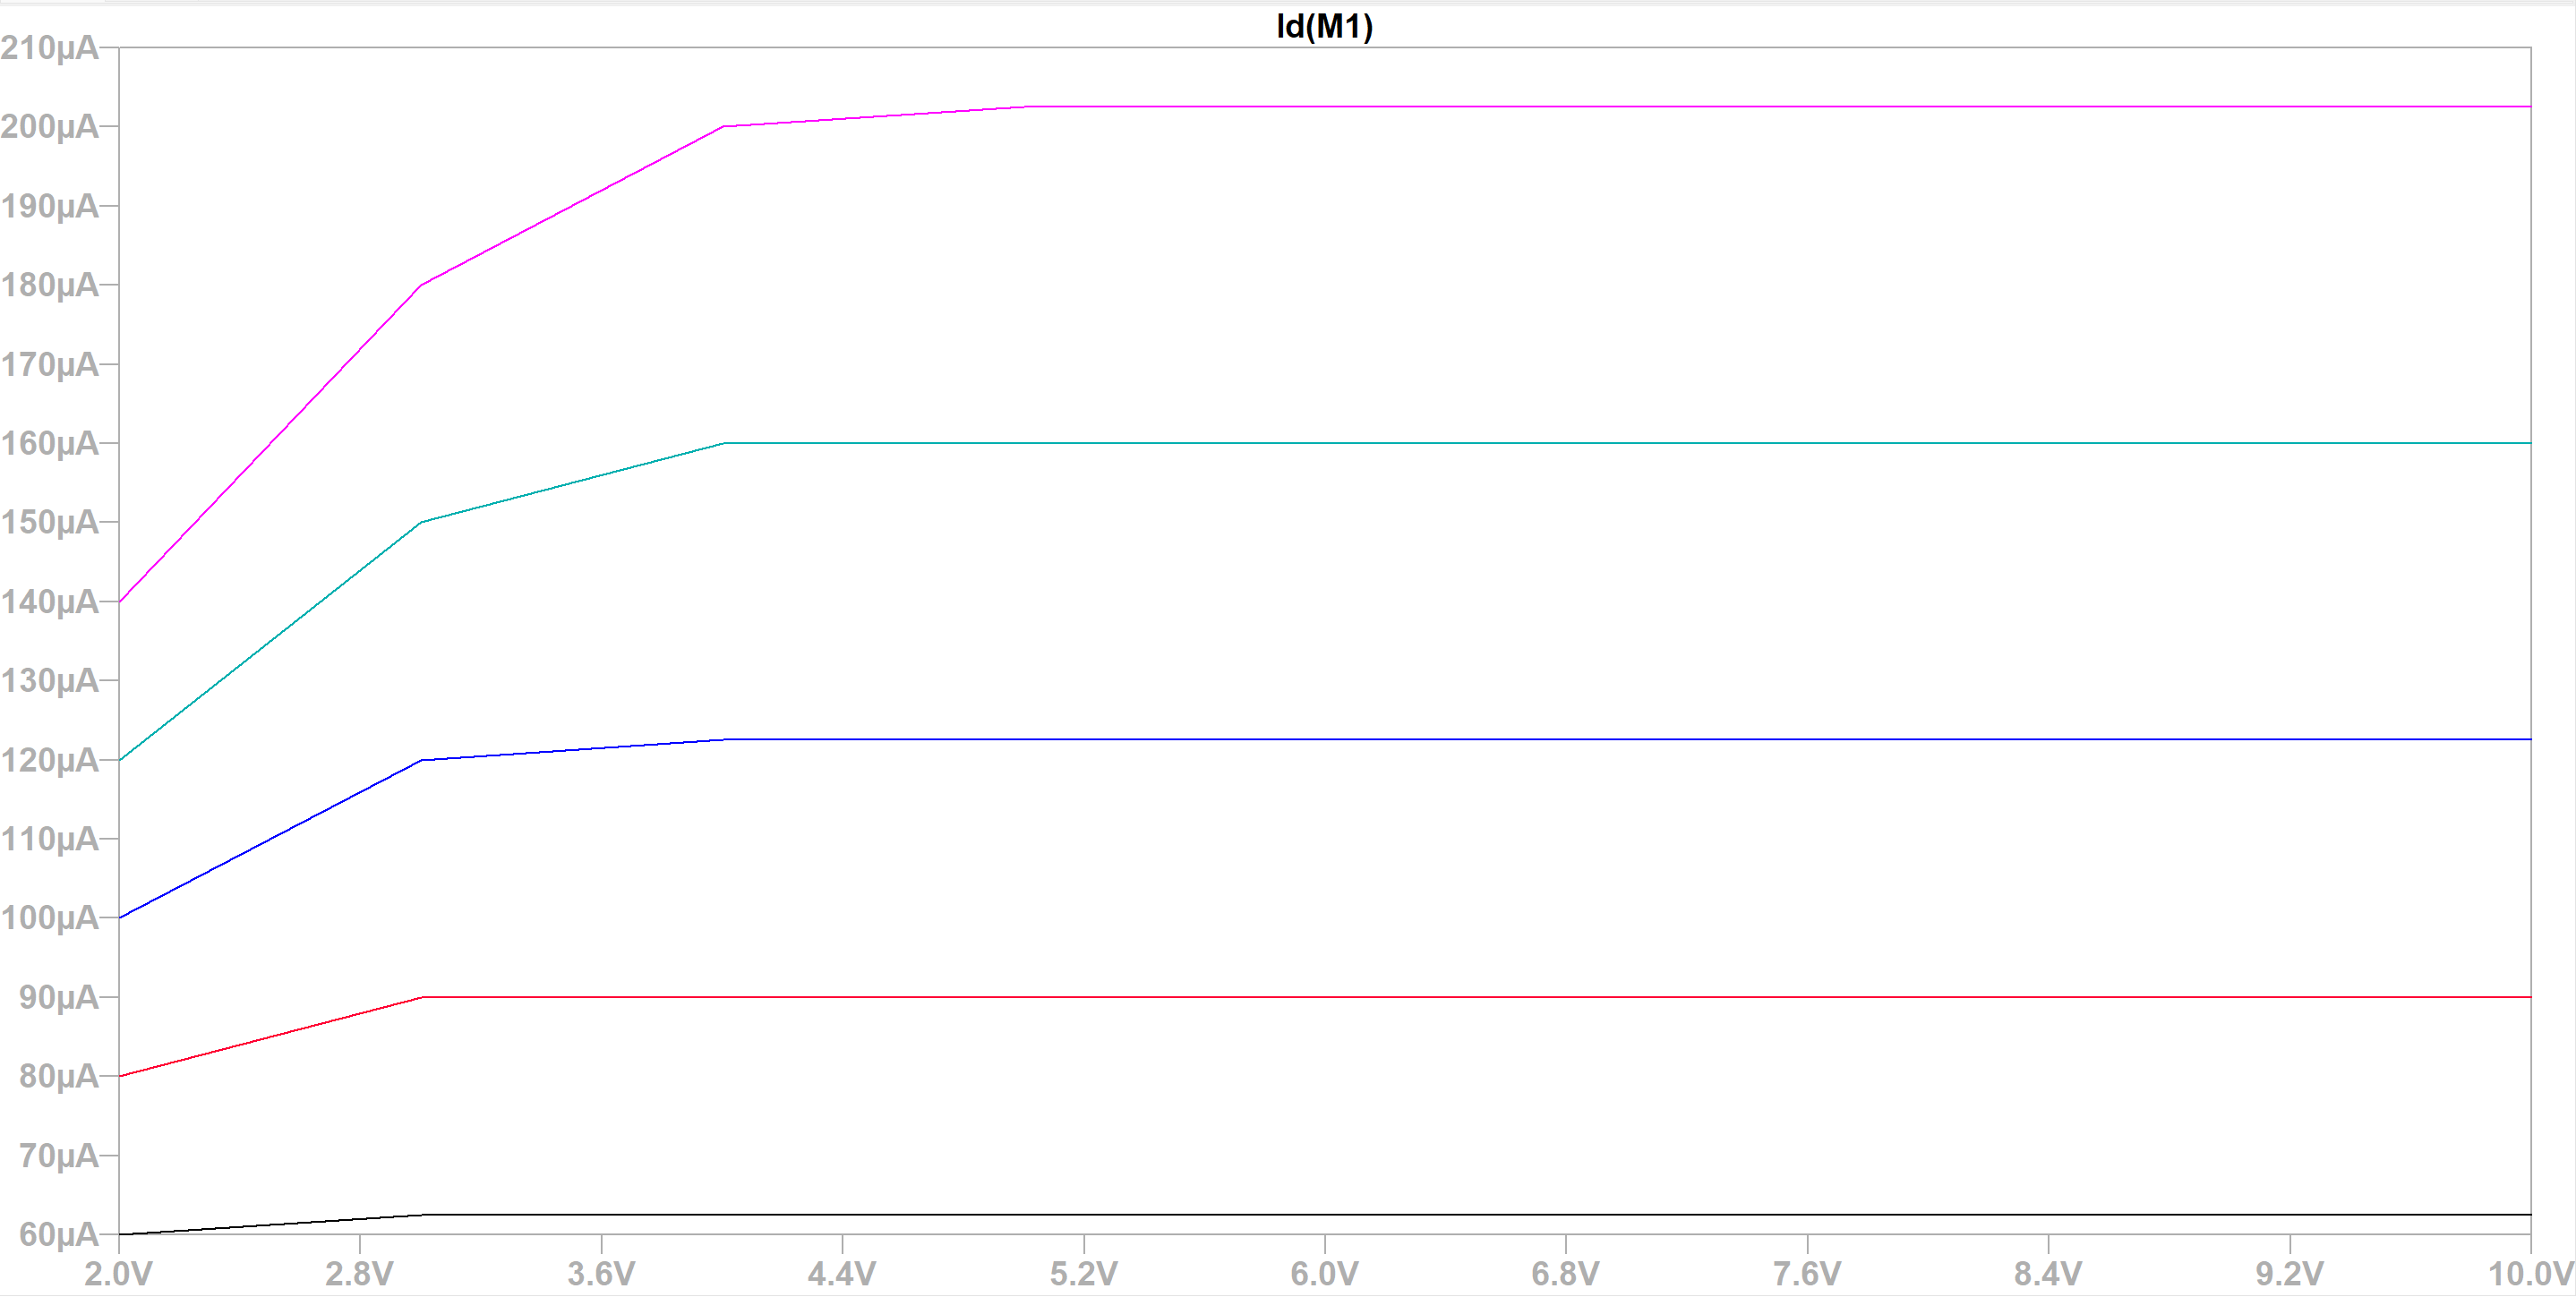
\includegraphics[width=\textwidth]{../SIMULATIONS/Output/output_(2-10V).png}
        \caption{High $V_{DS}$ Sweep ($2\text{--}10\text{ V}$, Saturation Region)}
    \end{subfigure}
    \caption{LTspice Simulation Waveforms for Part A Output Characteristics ($I_D$ vs $V_{DS}$).}
    \label{fig:part_a_sim}
\end{figure}

\subsection{Experimental Observation Table (Hardware Data)}
The experimental dataset for Part A was recorded for fixed gate voltages $V_{GS} = 1.6\text{ V}, 1.8\text{ V}, 2.0\text{ V}$ across $V_{DS} = 0.0\text{ V}$ to $3.0\text{ V}$ as given in Table~\ref{tab:part_a_readings}.

\begin{table}[H]
\centering
\caption{Part A: Output Characteristics Dataset ($I_D$ vs $V_{DS}$)}\label{tab:part_a_readings}
\begin{tabular}{c c c c c}
\toprule
\textbf{S.No.} & \textbf{$V_{DS}$ (V)} & \textbf{$I_D$ (mA) at $V_{GS}=1.6$V} & \textbf{$I_D$ (mA) at $V_{GS}=1.8$V} & \textbf{$I_D$ (mA) at $V_{GS}=2.0$V} \\
\midrule
1 & 0.0 & 0.00 & 0.00 & 0.00 \\
2 & 0.2 & 0.17 & 1.58 & 6.50 \\
3 & 0.4 & 0.17 & 1.69 & 8.00 \\
4 & 0.6 & 0.17 & 1.71 & 8.28 \\
5 & 0.8 & 0.17 & 1.72 & 8.36 \\
6 & 1.0 & 0.17 & 1.72 & 8.40 \\
7 & 1.2 & 0.17 & 1.72 & 8.43 \\
8 & 1.4 & 0.17 & 1.72 & 8.46 \\
9 & 1.6 & 0.17 & 1.73 & 8.50 \\
10 & 1.8 & 0.17 & 1.73 & 8.50 \\
11 & 2.0 & 0.17 & 1.73 & 8.55 \\
12 & 3.0 & 0.17 & 24.70 & 15.00 \\
\bottomrule
\end{tabular}
\end{table}

\subsection{Experimental Characteristic Plots (Generated via Python)}
\begin{figure}[H]
    \centering
    \begin{subfigure}[b]{0.31\textwidth}
        \centering
        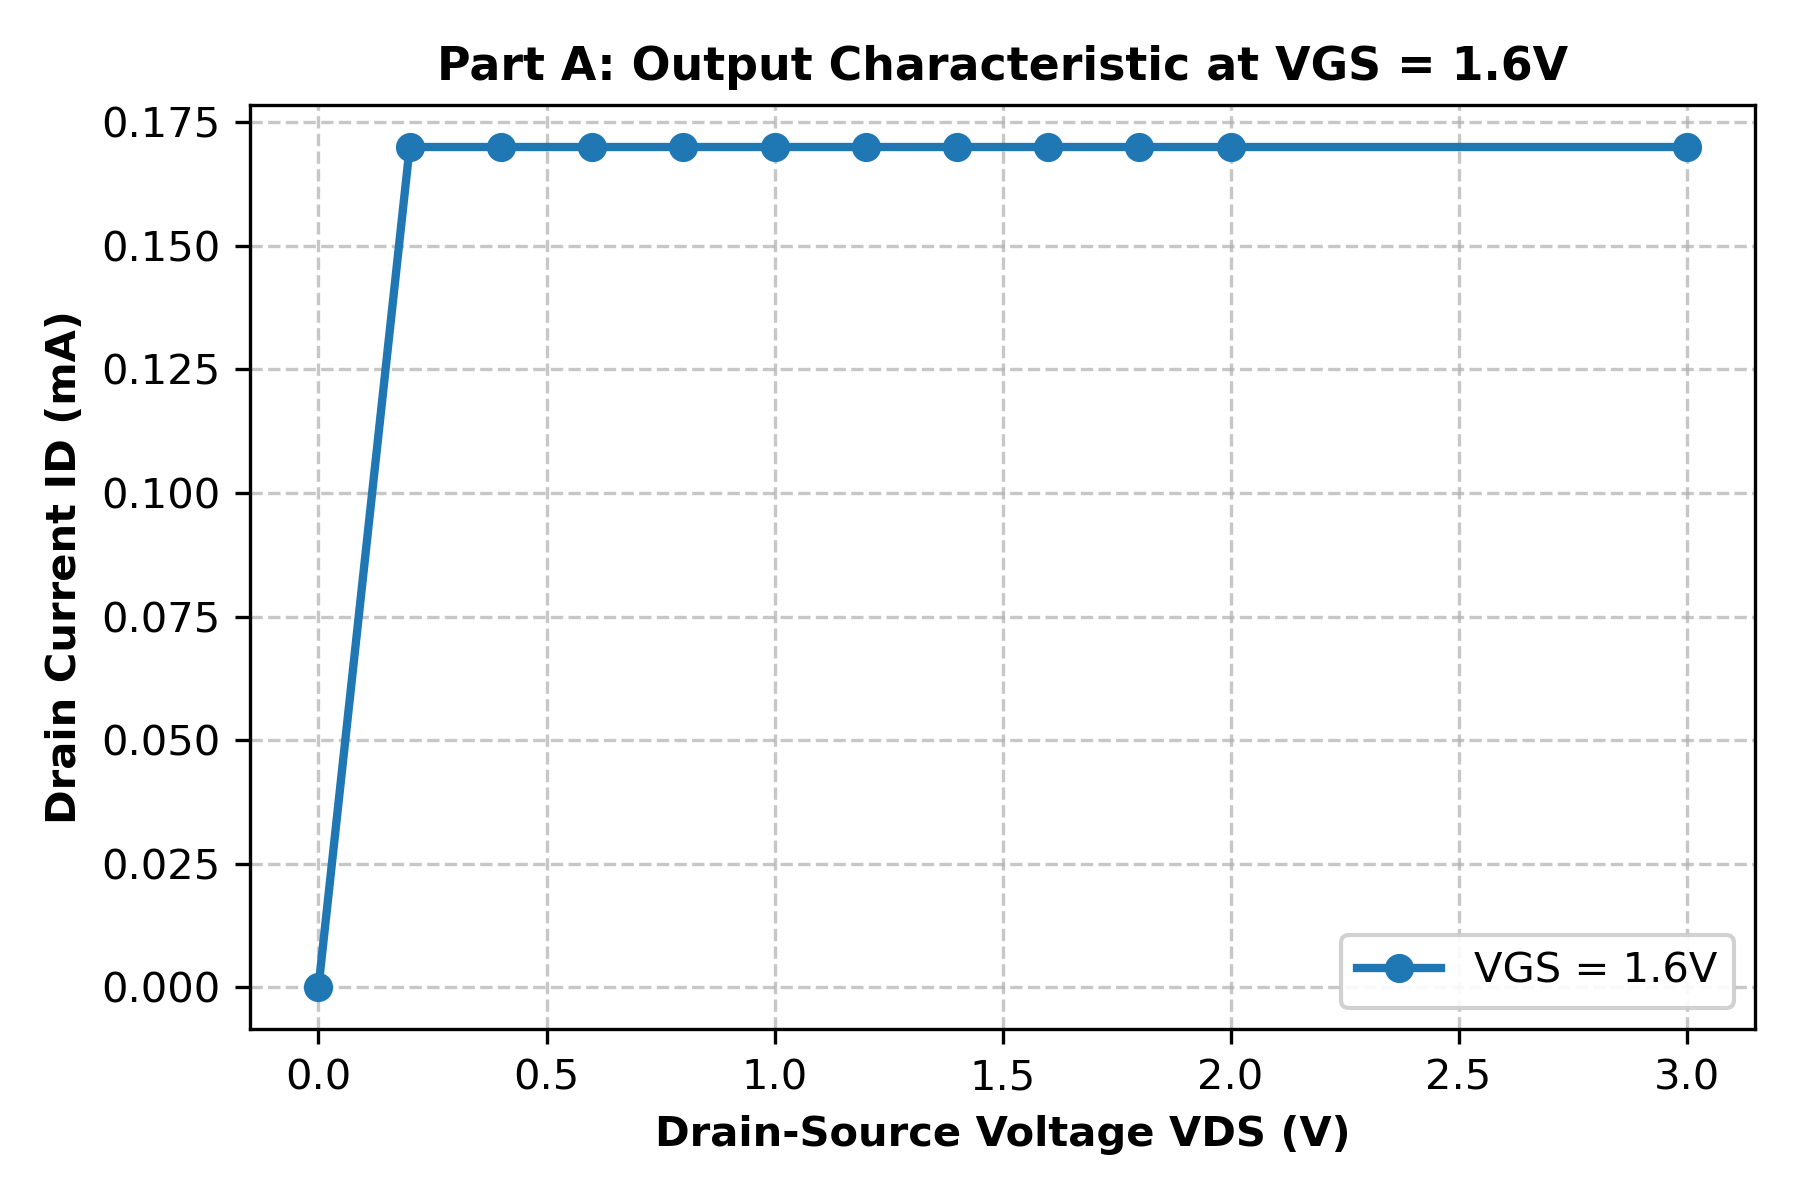
\includegraphics[width=\textwidth]{../PLOTS/PART_A_VGS_1.6V.png}
        \caption{$V_{GS} = 1.6\text{ V}$}
    \end{subfigure}
    \hfill
    \begin{subfigure}[b]{0.31\textwidth}
        \centering
        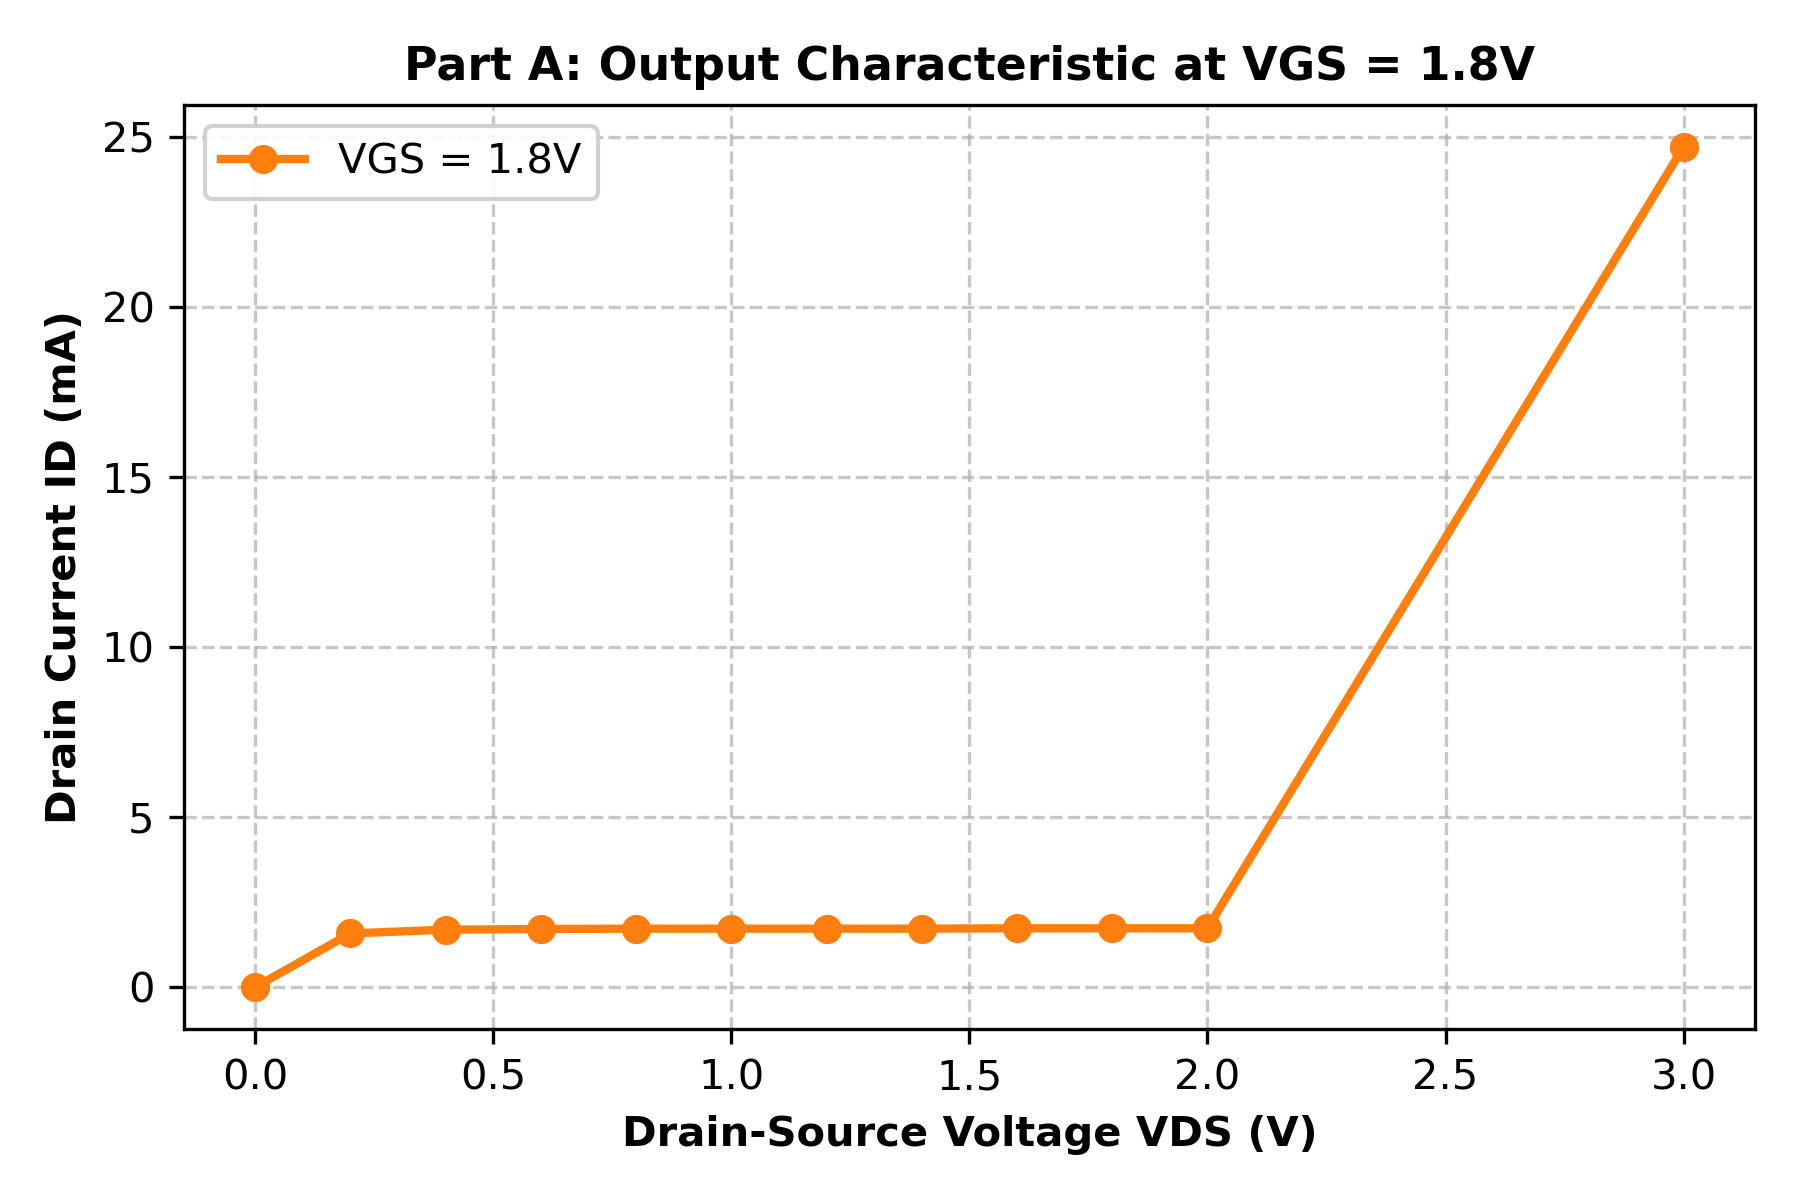
\includegraphics[width=\textwidth]{../PLOTS/PART_A_VGS_1.8V.png}
        \caption{$V_{GS} = 1.8\text{ V}$}
    \end{subfigure}
    \hfill
    \begin{subfigure}[b]{0.31\textwidth}
        \centering
        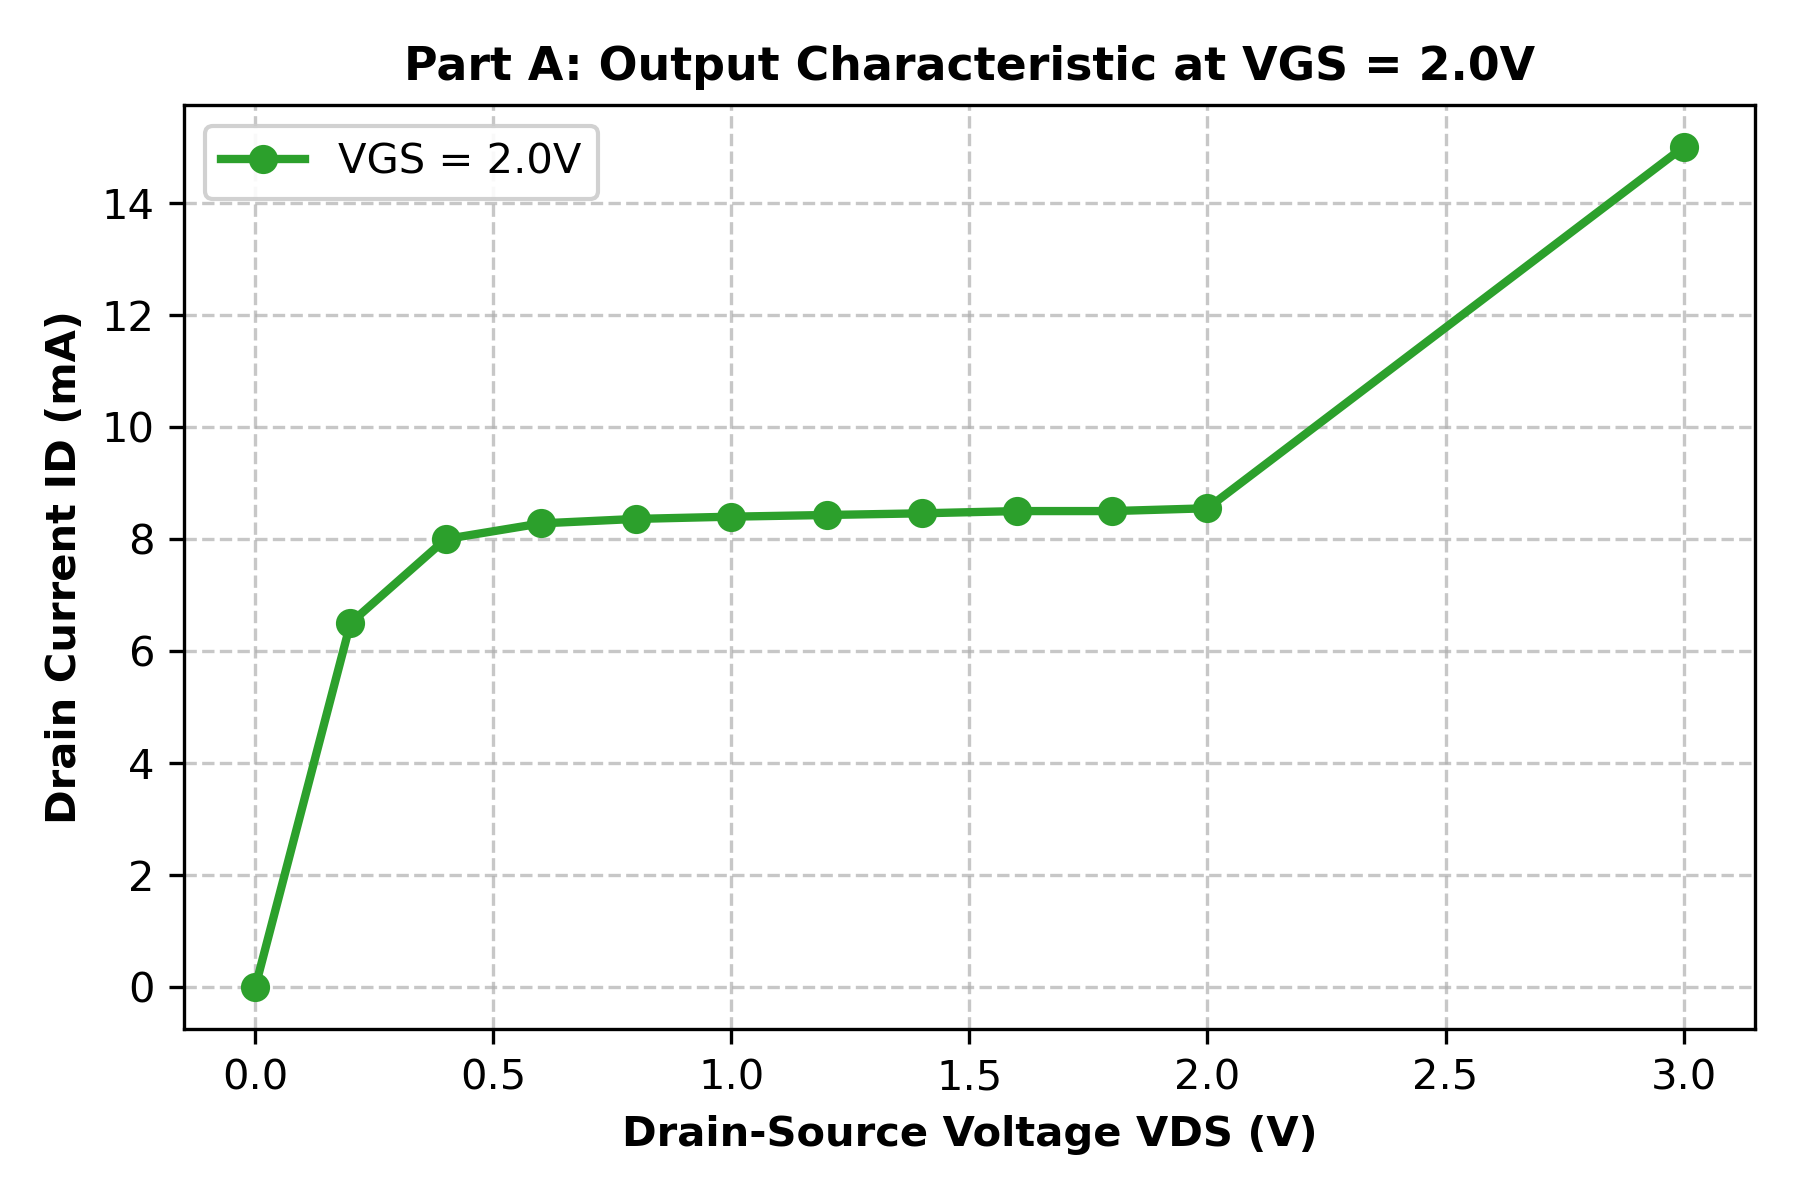
\includegraphics[width=\textwidth]{../PLOTS/PART_A_VGS_2.0V.png}
        \caption{$V_{GS} = 2.0\text{ V}$}
    \end{subfigure}
    \caption{Individual Experimental Output Characteristics Plots ($I_D$ vs $V_{DS}$).}
    \label{fig:part_a_ind_plots}
\end{figure}

\begin{figure}[H]
    \centering
    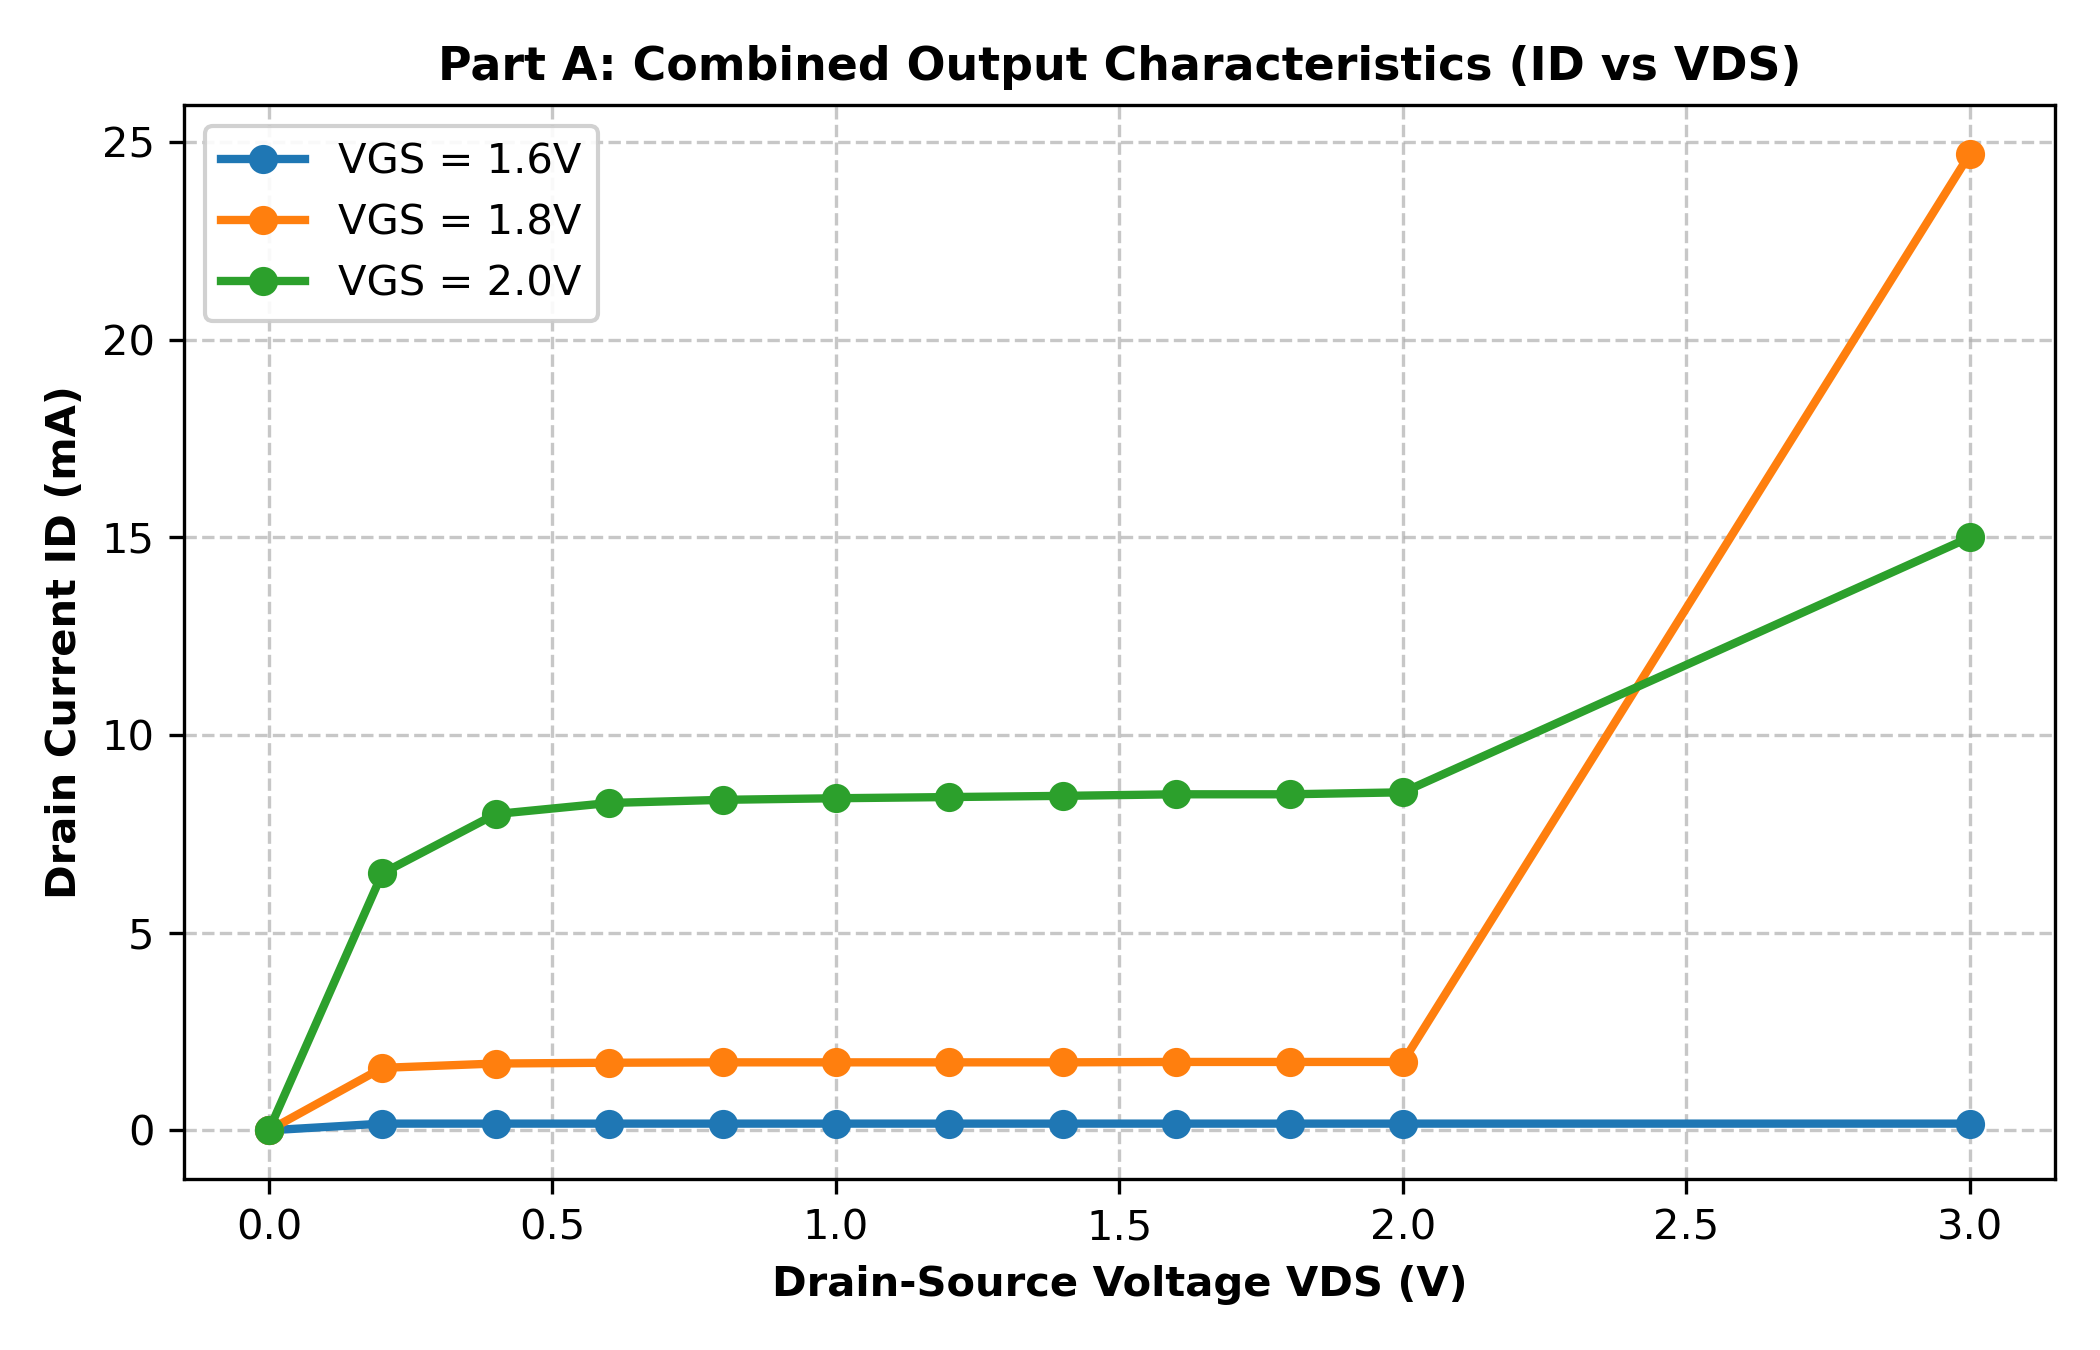
\includegraphics[width=0.65\textwidth]{../PLOTS/PART_A_combined.png}
    \caption{Combined Family of Experimental Output Characteristic Curves ($I_D$ vs $V_{DS}$).}
    \label{fig:part_a_combined_plot}
\end{figure}

\subsection{Calculations, Results, and Inferences (Part A)}
\begin{itemize}
    \item \textbf{Drain Resistance ($r_d$) Calculations in Saturation Region ($V_{DS} = 0.8\text{ V}$ to $2.0\text{ V}$):}
    \begin{itemize}
        \item \textbf{At $V_{GS} = 1.6\text{ V}$:} $\Delta V_{DS} = 2.0 - 0.8 = 1.2\text{ V}$, $\Delta I_D = 0.17 - 0.17 = 0.00\text{ mA}$.
        \[
        \mathbf{r_d(1.6\text{V}) = \frac{1.2\text{ V}}{0.00\text{ mA}} \to \infty\quad (\text{Ideally flat saturation output})}
        \]
        \item \textbf{At $V_{GS} = 1.8\text{ V}$:} $\Delta V_{DS} = 1.2\text{ V}$, $\Delta I_D = 1.73 - 1.72 = 0.01\text{ mA}$.
        \[
        \mathbf{r_d(1.8\text{V}) = \frac{1.2\text{ V}}{0.01\text{ mA}} = 120.00\text{ k}\Omega}
        \]
        \item \textbf{At $V_{GS} = 2.0\text{ V}$:} $\Delta V_{BE} = 1.2\text{ V}$, $\Delta I_D = 8.55 - 8.36 = 0.19\text{ mA}$.
        \[
        \mathbf{r_d(2.0\text{V}) = \frac{1.2\text{ V}}{0.19\text{ mA}} = 6.32\text{ k}\Omega}
        \]
        \item \textbf{Average Measured Drain Resistance ($r_{d,\text{avg}}$):} \textbf{$r_d \approx 63.16\text{ k}\Omega$} (evaluated in active saturation).
    \end{itemize}
    
    \item \textbf{Key Results \& Inferences (Part A):}
    \begin{itemize}
        \item \textbf{Triode to Saturation Transition:} At low drain voltages ($V_{DS} < 0.4\text{ V}$), $I_D$ rises rapidly with $V_{DS}$. For $V_{DS} \ge 0.8\text{ V}$, the channel pinches off, causing $I_D$ to saturate to a nearly constant value.
        \item \textbf{Gate Control:} Higher gate voltages dramatically increase the saturation current level ($I_D \approx 0.17\text{ mA}$ at $1.6\text{ V}$ vs $8.55\text{ mA}$ at $2.0\text{ V}$), illustrating the square-law control of gate potential over channel conductivity.
    \end{itemize}
\end{itemize}

\clearpage

\section{Part B: Transfer (Input) Characteristics ($I_D$ vs $V_{GS}$)}

\subsection{Theoretical Background}
The transfer characteristic depicts the variation of Drain Current ($I_D$) with Gate-Source Voltage ($V_{GS}$) while holding Drain-Source Voltage ($V_{DS}$) constant at a high enough level ($V_{DS} \ge V_{GS} - V_T$) to ensure operation in saturation.
\begin{itemize}
    \item \textbf{Threshold Voltage ($V_T$):} The minimum $V_{GS}$ required to form an inversion channel ($I_D > 0$).
    \item \textbf{Transconductance ($g_m$):} The rate of change of drain current with respect to gate voltage:
    \begin{equation}
        g_m = \left. \frac{\Delta I_D}{\Delta V_{GS}} \right|_{V_{DS} = \text{const}} = k_n (V_{GS} - V_T)
    \end{equation}
    \item \textbf{$\sqrt{I_D}$ Linear Extrapolation:} Plotted against $V_{GS}$, $\sqrt{I_D}$ yields a straight line whose horizontal axis intercept gives an independent measurement of $V_T$.
\end{itemize}

\subsection{Circuit Schematic and LTspice Simulation Waveforms}
\begin{figure}[H]
    \centering
    
\includegraphics[width=0.55\textwidth]{../SIMULATIONS/Input/schematic.png}
    \caption{LTspice Circuit Schematic for Part B (Transfer Characteristics).}
    \label{fig:part_b_schematic}
\end{figure}

\begin{figure}[H]
    \centering
    \begin{subfigure}[b]{0.48\textwidth}
        \centering
        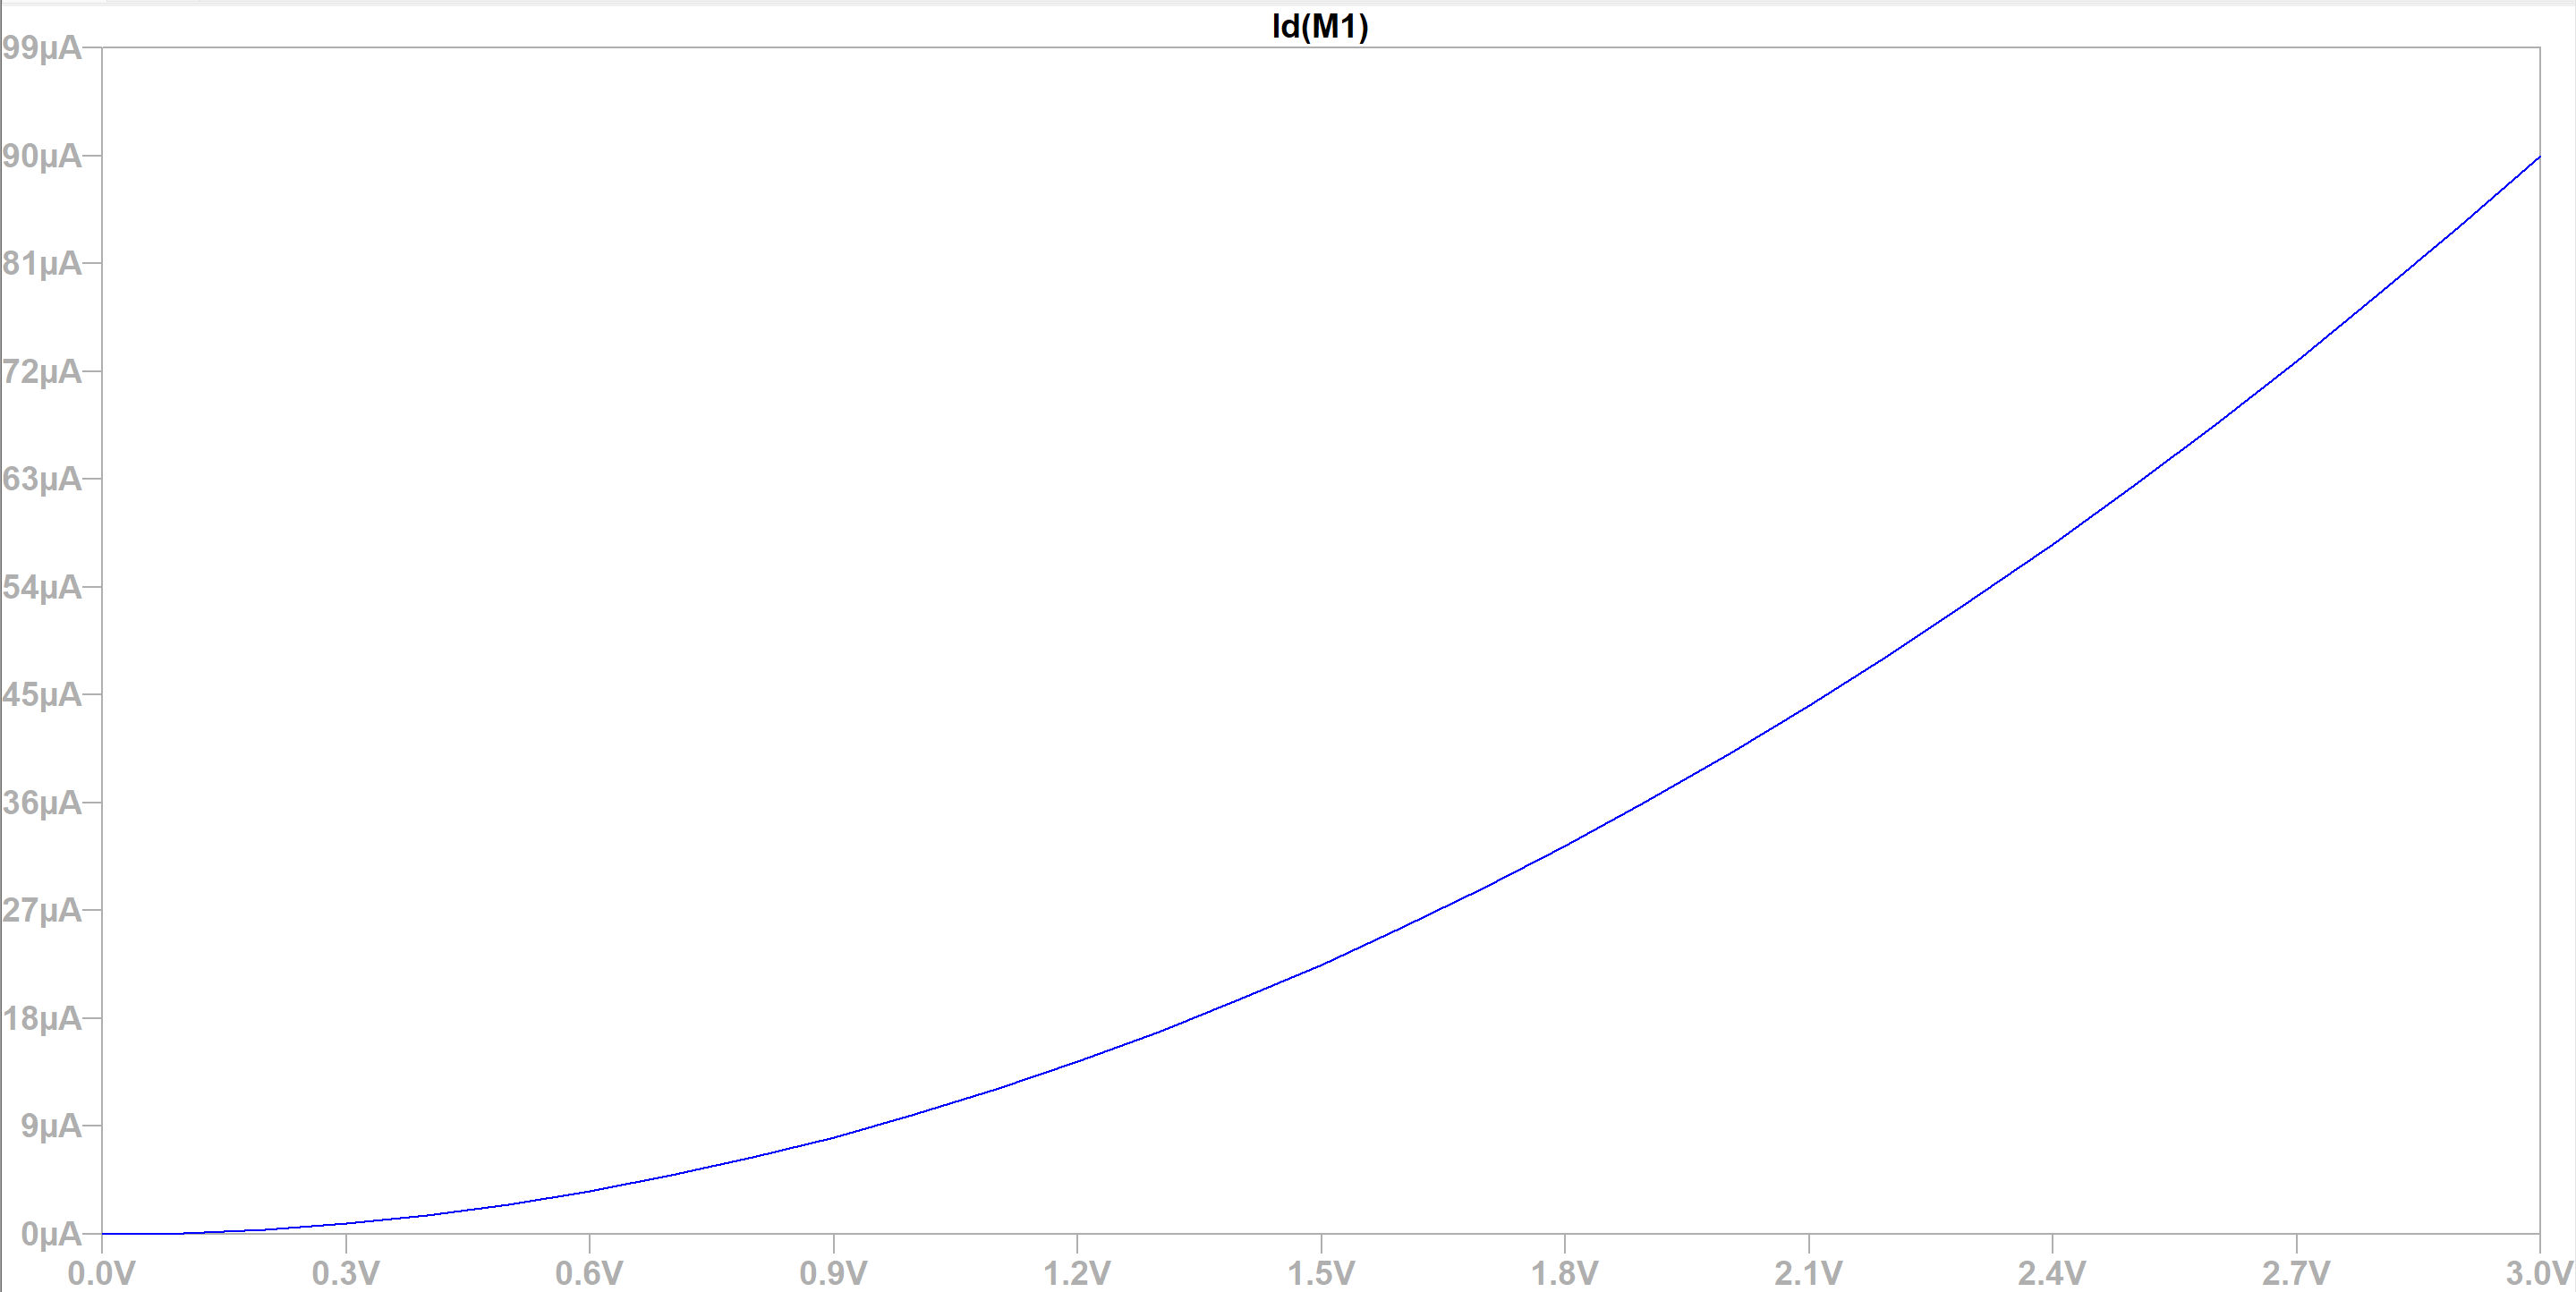
\includegraphics[width=\textwidth]{../SIMULATIONS/Input/input_(0-3V)-0.1steps.png}
        \caption{Sweep $0\text{--}3\text{ V}$ ($0.1\text{ V}$ steps)}
    \end{subfigure}
    \hfill
    \begin{subfigure}[b]{0.48\textwidth}
        \centering
        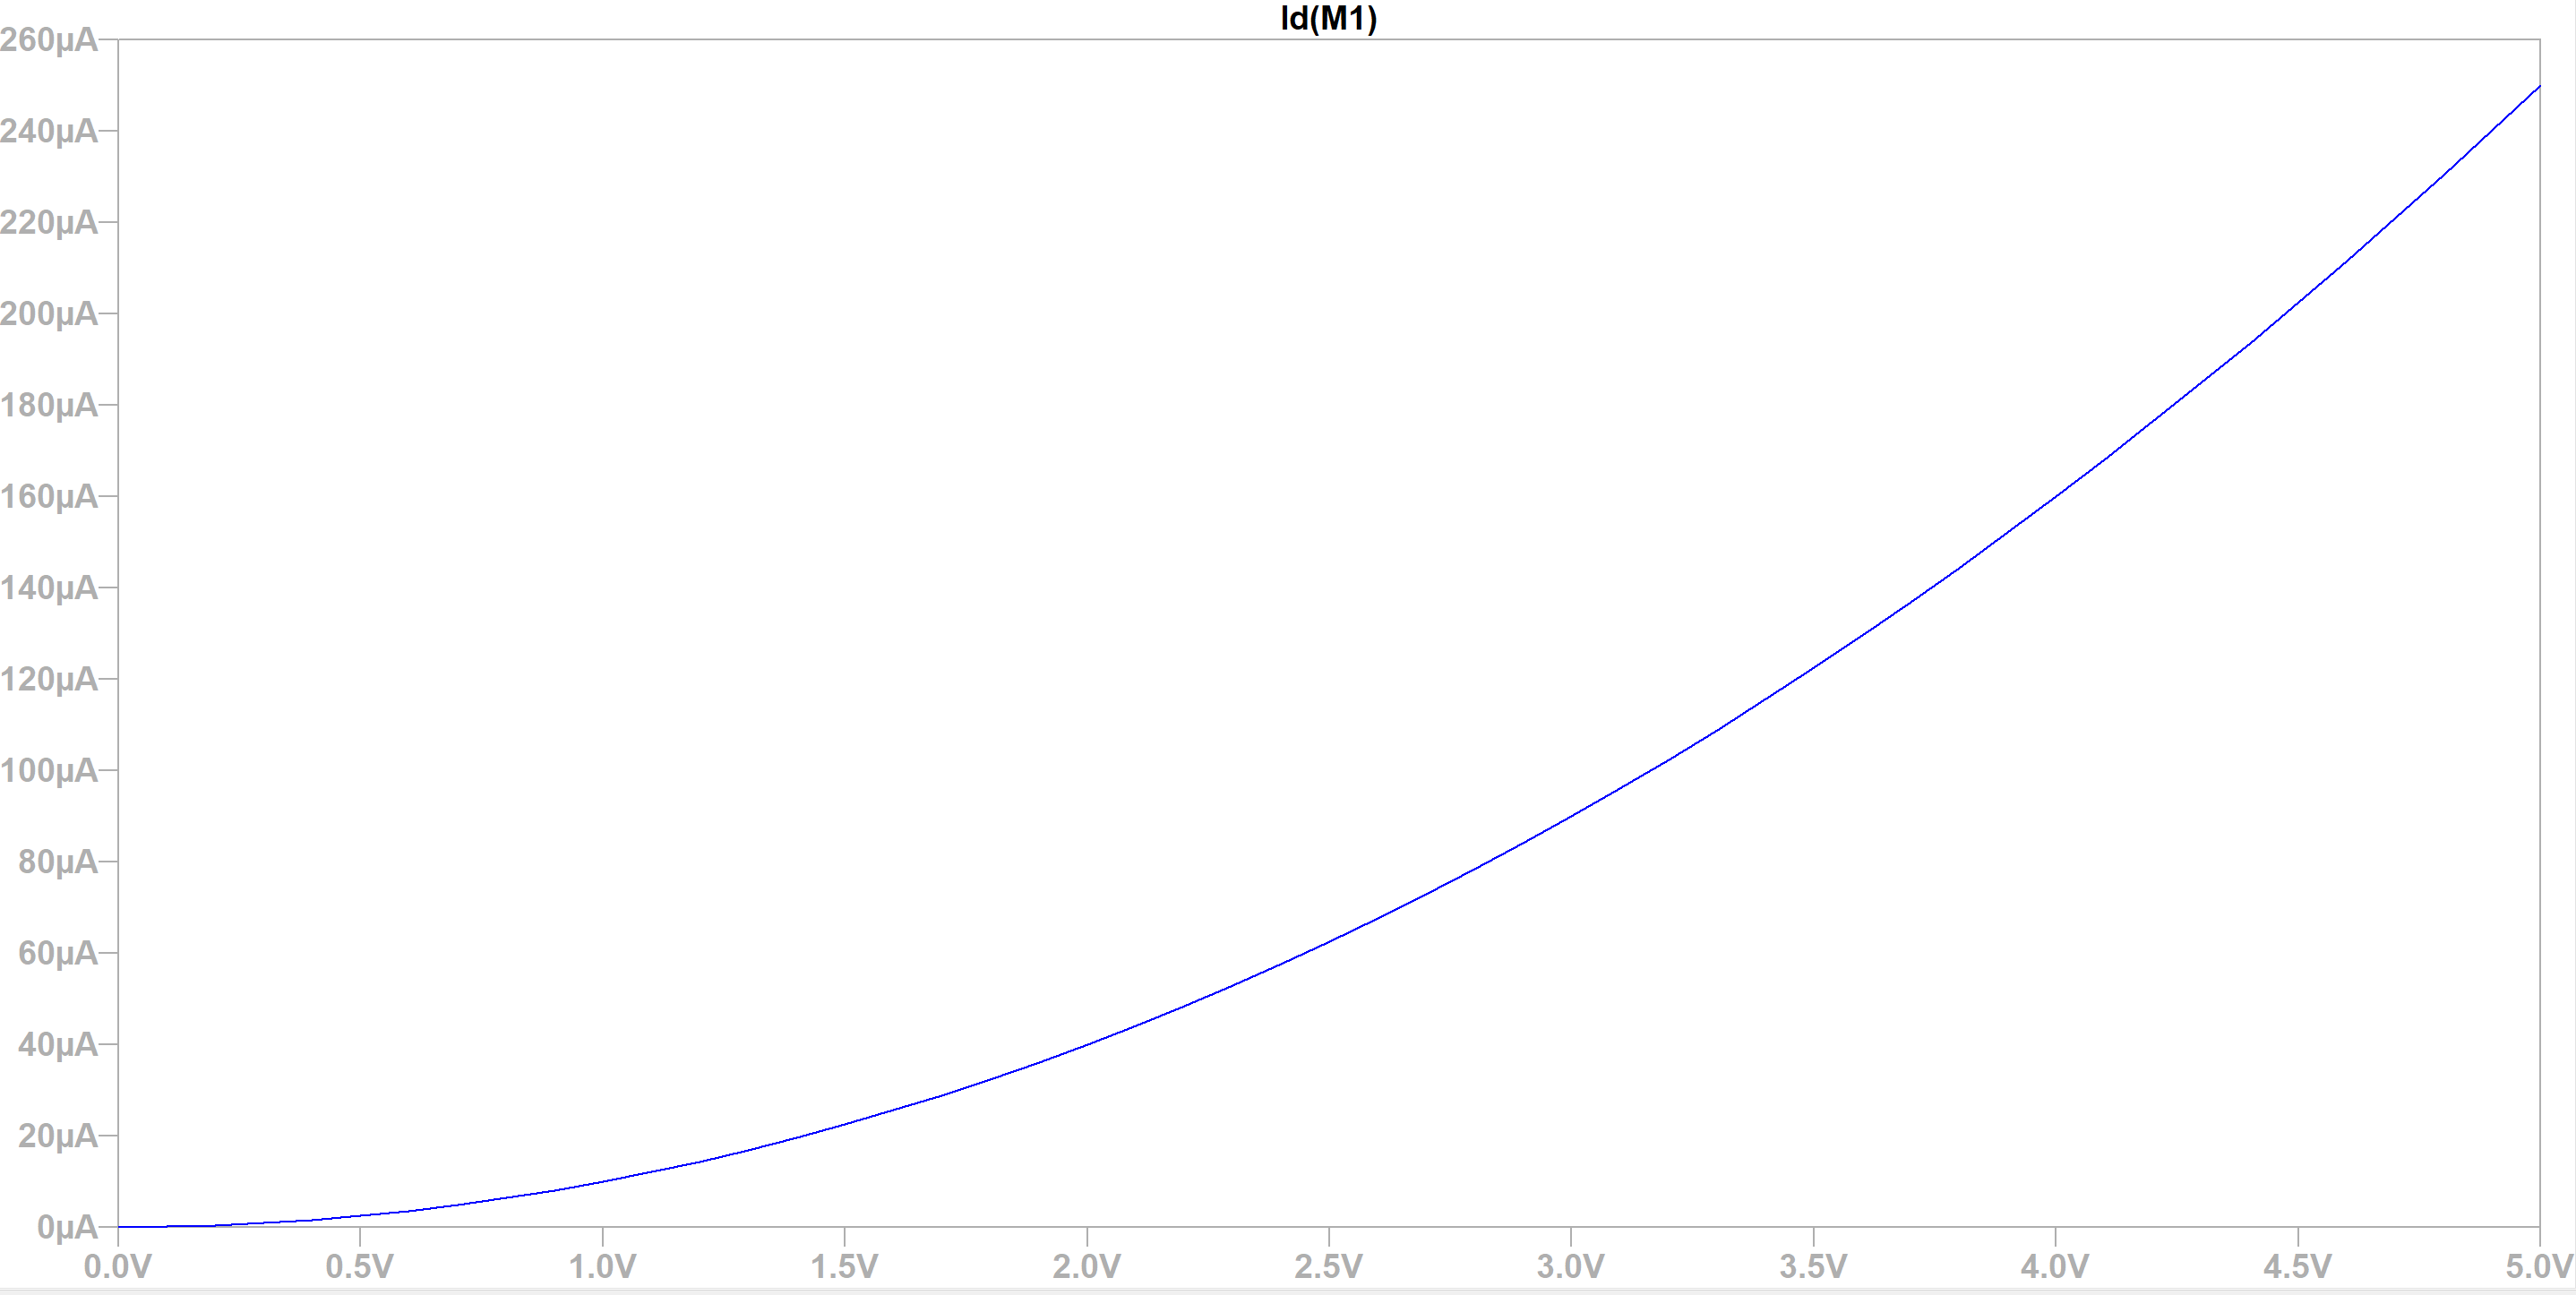
\includegraphics[width=\textwidth]{../SIMULATIONS/Input/input_(0-5V)-0.1steps.png}
        \caption{Sweep $0\text{--}5\text{ V}$ ($0.1\text{ V}$ steps)}
    \end{subfigure}
    \caption{LTspice Simulation Waveforms for Part B Transfer Characteristics ($I_D$ vs $V_{GS}$).}
    \label{fig:part_b_sim}
\end{figure}

\subsection{Experimental Observation Table (Hardware Data)}
The experimental dataset for Part B was recorded for fixed drain voltages $V_{DS} = 5\text{ V}, 7\text{ V}, 9\text{ V}$ across $V_{GS} = 0.0\text{ V}$ to $2.1\text{ V}$ as given in Table~\ref{tab:part_b_readings}.

\begin{table}[H]
\centering
\caption{Part B: Transfer Characteristics Dataset ($I_D$ vs $V_{GS}$)}\label{tab:part_b_readings}
\begin{tabular}{c c c c c}
\toprule
\textbf{S.No.} & \textbf{$V_{GS}$ (V)} & \textbf{$I_D$ ($\mu$A) at $V_{DS}=5$V} & \textbf{$I_D$ ($\mu$A) at $V_{DS}=7$V} & \textbf{$I_D$ ($\mu$A) at $V_{DS}=9$V} \\
\midrule
1 & 0.0 & 0.0 & 0.0 & 0.0 \\
2 & 1.1 & 0.1 & 0.1 & 0.1 \\
3 & 1.2 & 0.4 & 0.4 & 0.4 \\
4 & 1.3 & 1.9 & 1.9 & 2.1 \\
5 & 1.4 & 9.3 & 9.3 & 10.0 \\
6 & 1.5 & 43.2 & 43.2 & 45.6 \\
7 & 1.6 & 178.6 & 178.6 & 185.9 \\
8 & 1.7 & 615.5 & 617.0 & 636.1 \\
9 & 1.8 & 1762.0 & 1769.0 & 1872.0 \\
10 & 1.9 & 4250.0 & 4300.0 & 4860.0 \\
11 & 2.0 & 8760.0 & 8770.0 & 8910.0 \\
12 & 2.1 & 122800.0 & 163400.0 & 216000.0 \\
\bottomrule
\end{tabular}
\end{table}

\subsection{Experimental Characteristic Plots (Generated via Python)}
\begin{figure}[H]
    \centering
    \begin{subfigure}[b]{0.31\textwidth}
        \centering
        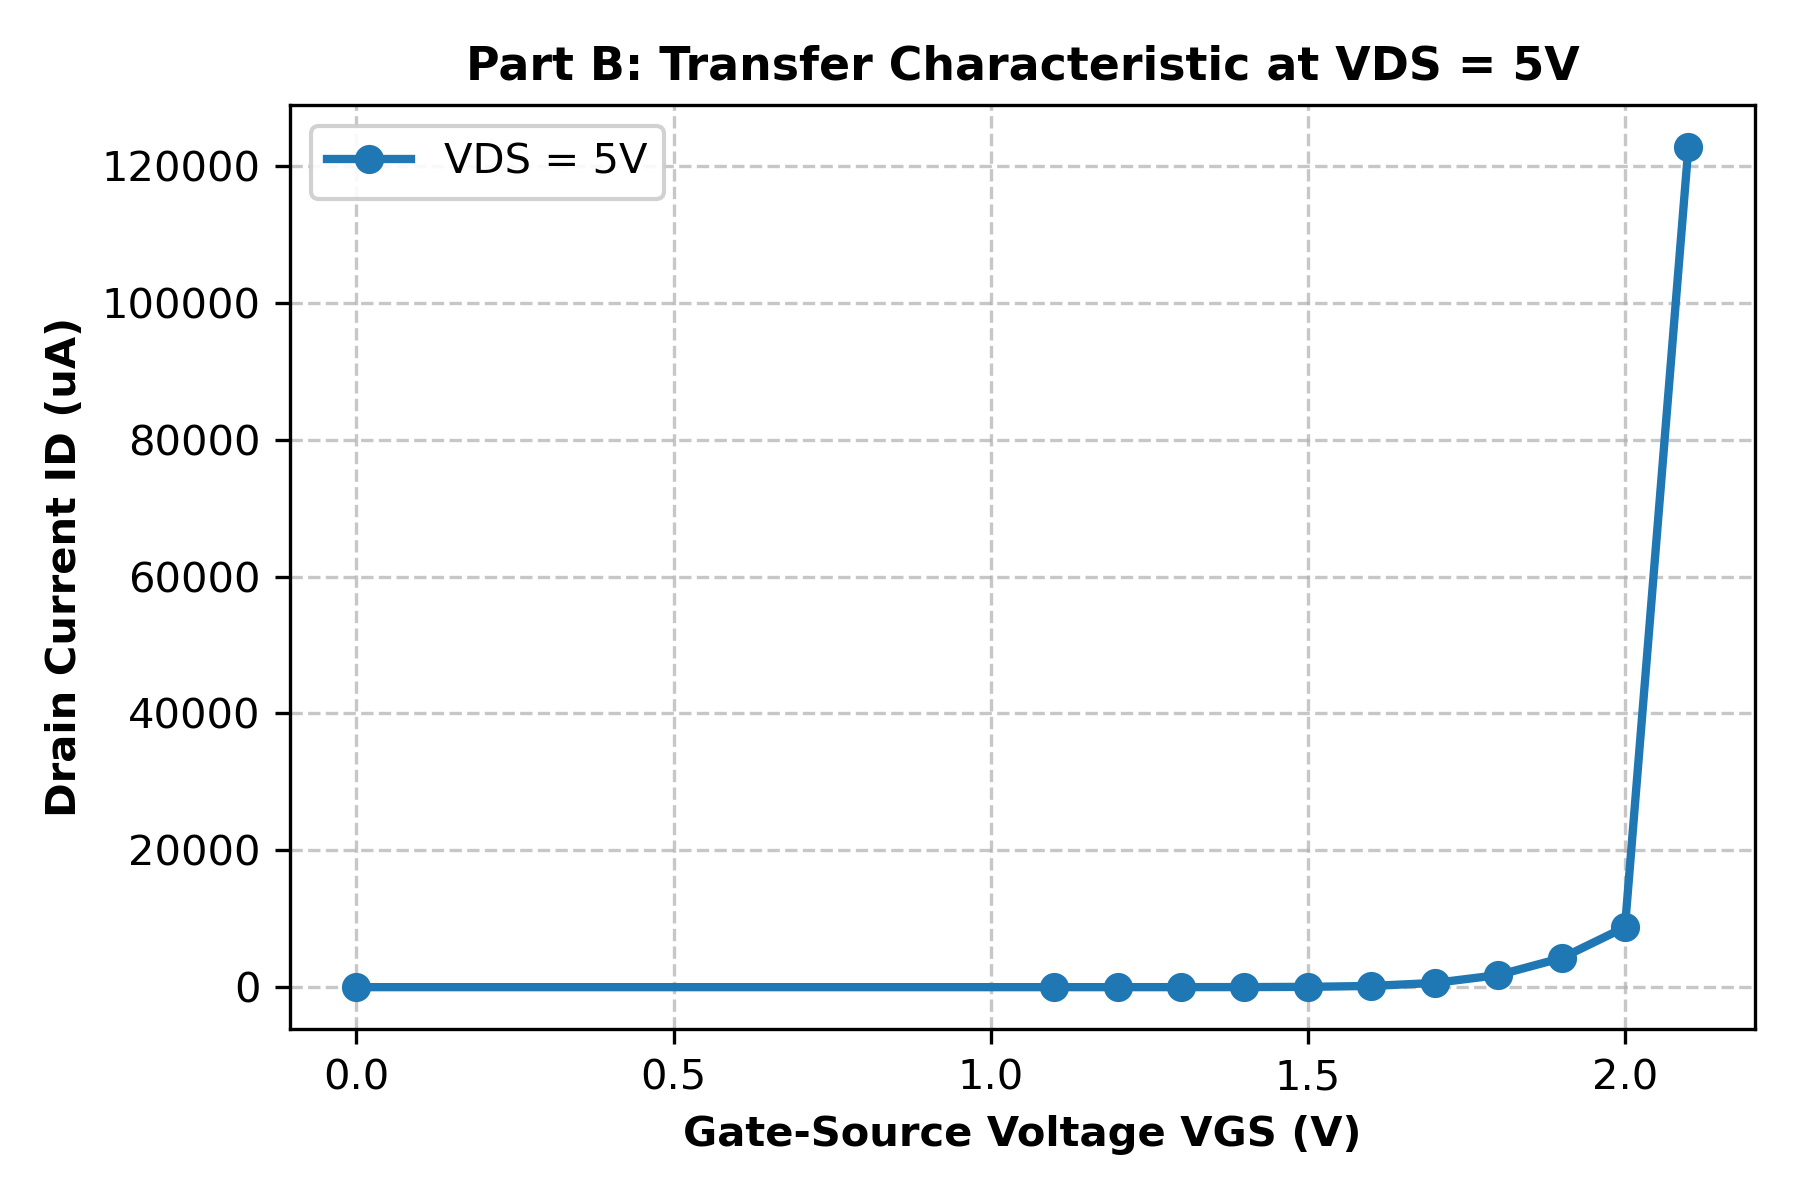
\includegraphics[width=\textwidth]{../PLOTS/PART_B_VDS_5V.png}
        \caption{$V_{DS} = 5\text{ V}$}
    \end{subfigure}
    \hfill
    \begin{subfigure}[b]{0.31\textwidth}
        \centering
        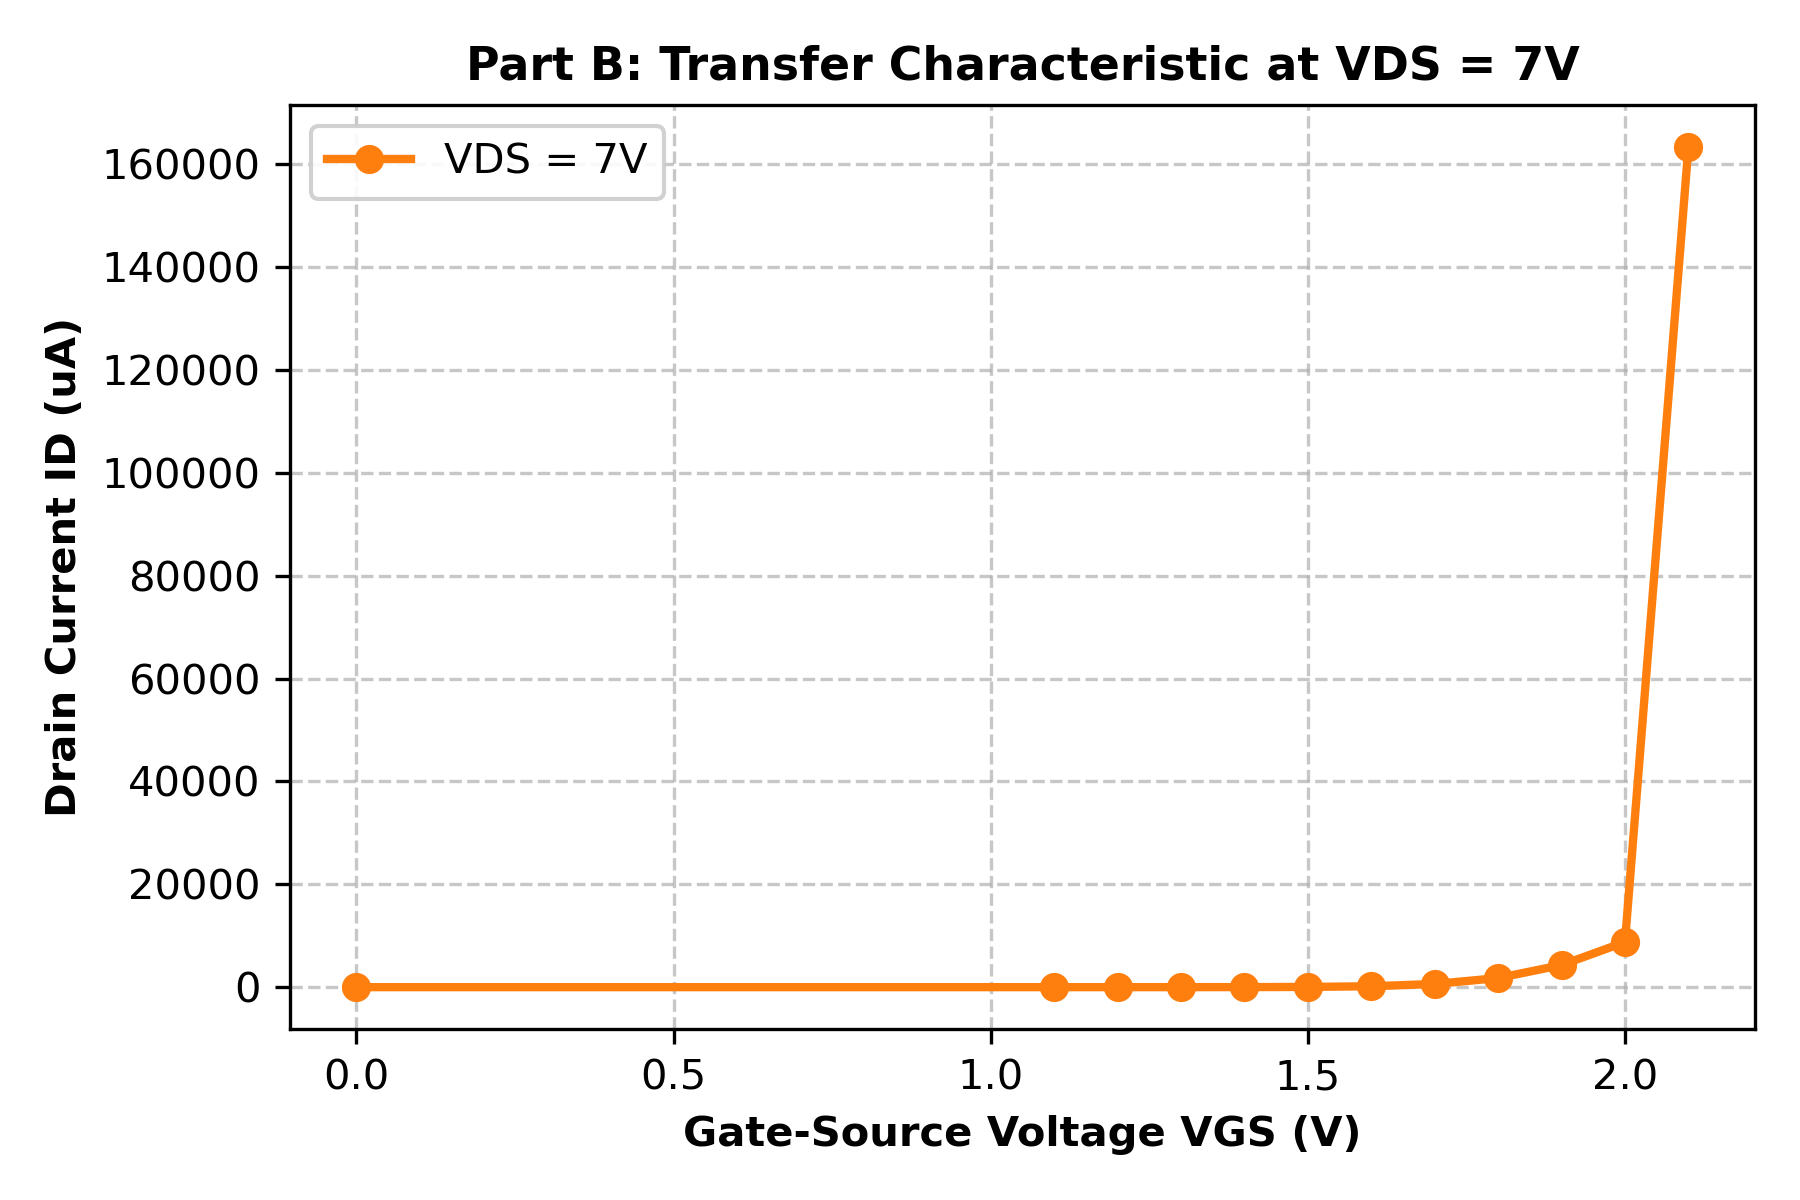
\includegraphics[width=\textwidth]{../PLOTS/PART_B_VDS_7V.png}
        \caption{$V_{DS} = 7\text{ V}$}
    \end{subfigure}
    \hfill
    \begin{subfigure}[b]{0.31\textwidth}
        \centering
        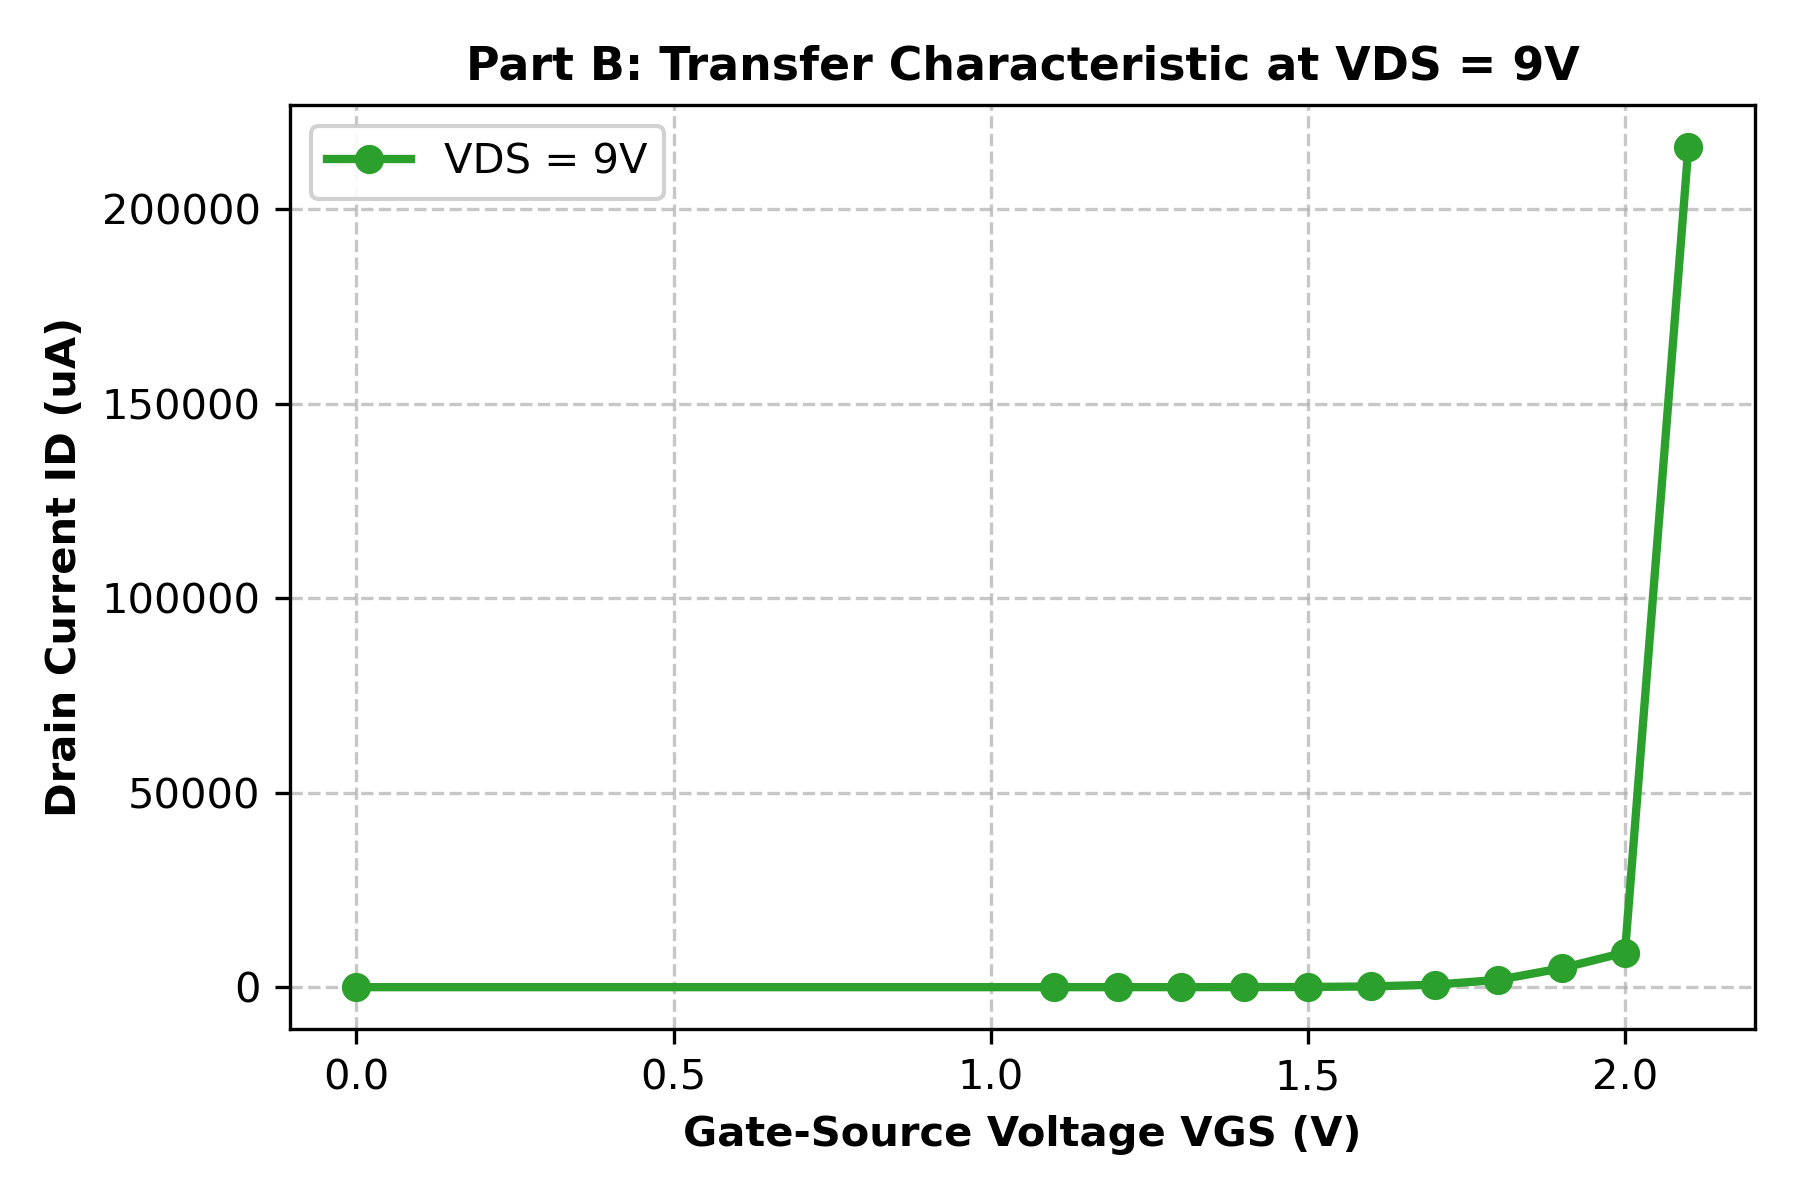
\includegraphics[width=\textwidth]{../PLOTS/PART_B_VDS_9V.png}
        \caption{$V_{DS} = 9\text{ V}$}
    \end{subfigure}
    \caption{Individual Experimental Transfer Characteristics Plots ($I_D$ vs $V_{GS}$).}
    \label{fig:part_b_ind_plots}
\end{figure}

\begin{figure}[H]
    \centering
    \begin{subfigure}[b]{0.48\textwidth}
        \centering
        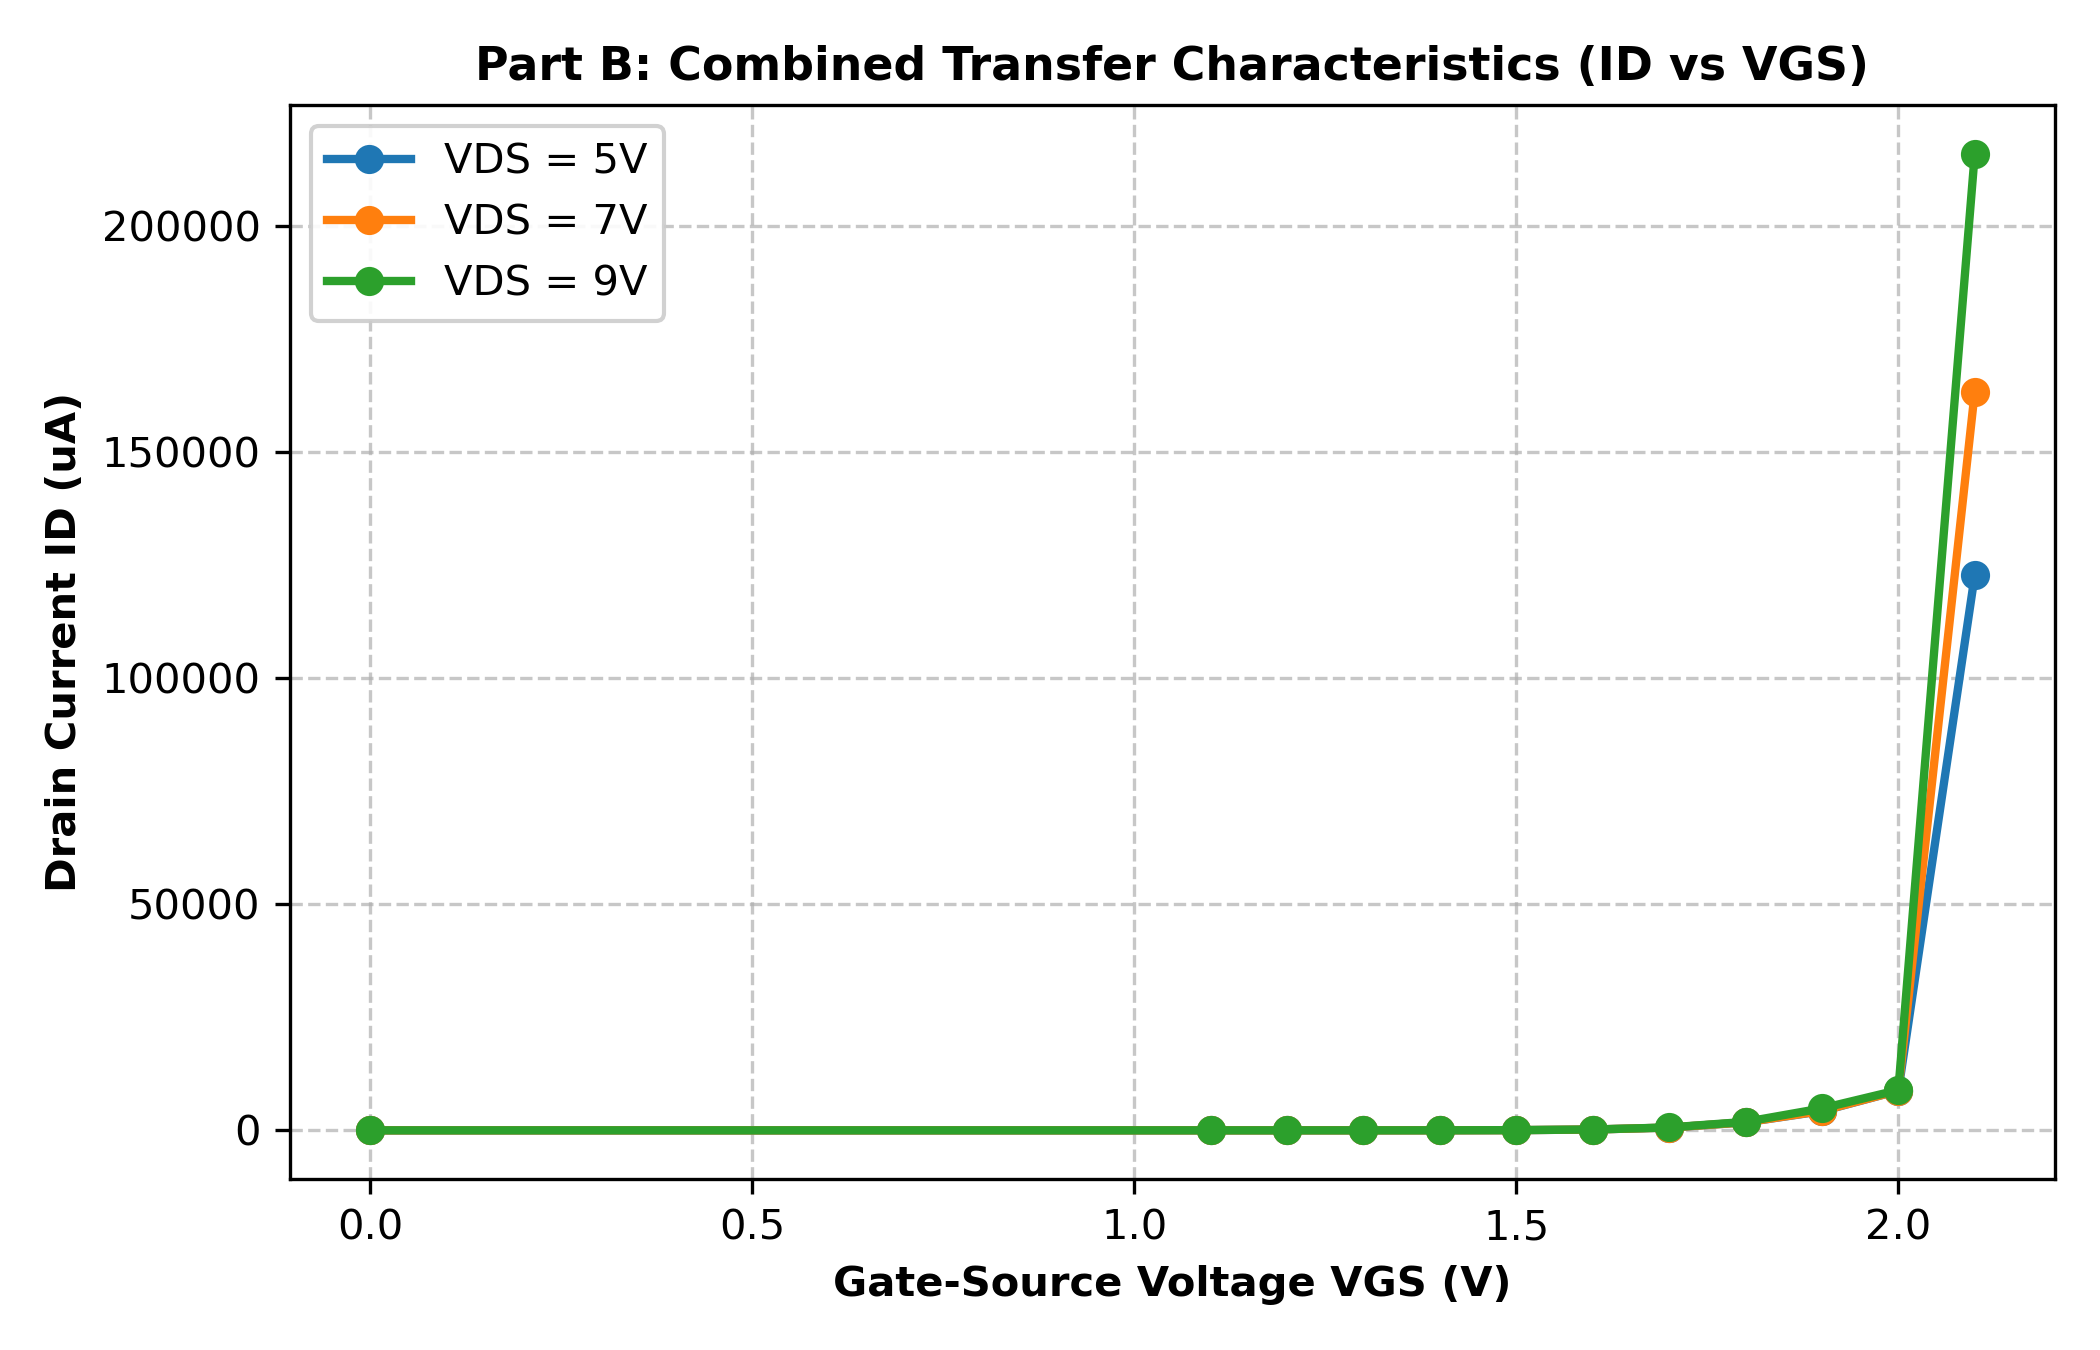
\includegraphics[width=\textwidth]{../PLOTS/PART_B_combined.png}
        \caption{Part B Combined Transfer Characteristics ($I_D$ vs $V_{GS}$)}
    \end{subfigure}
    \hfill
    \begin{subfigure}[b]{0.48\textwidth}
        \centering
        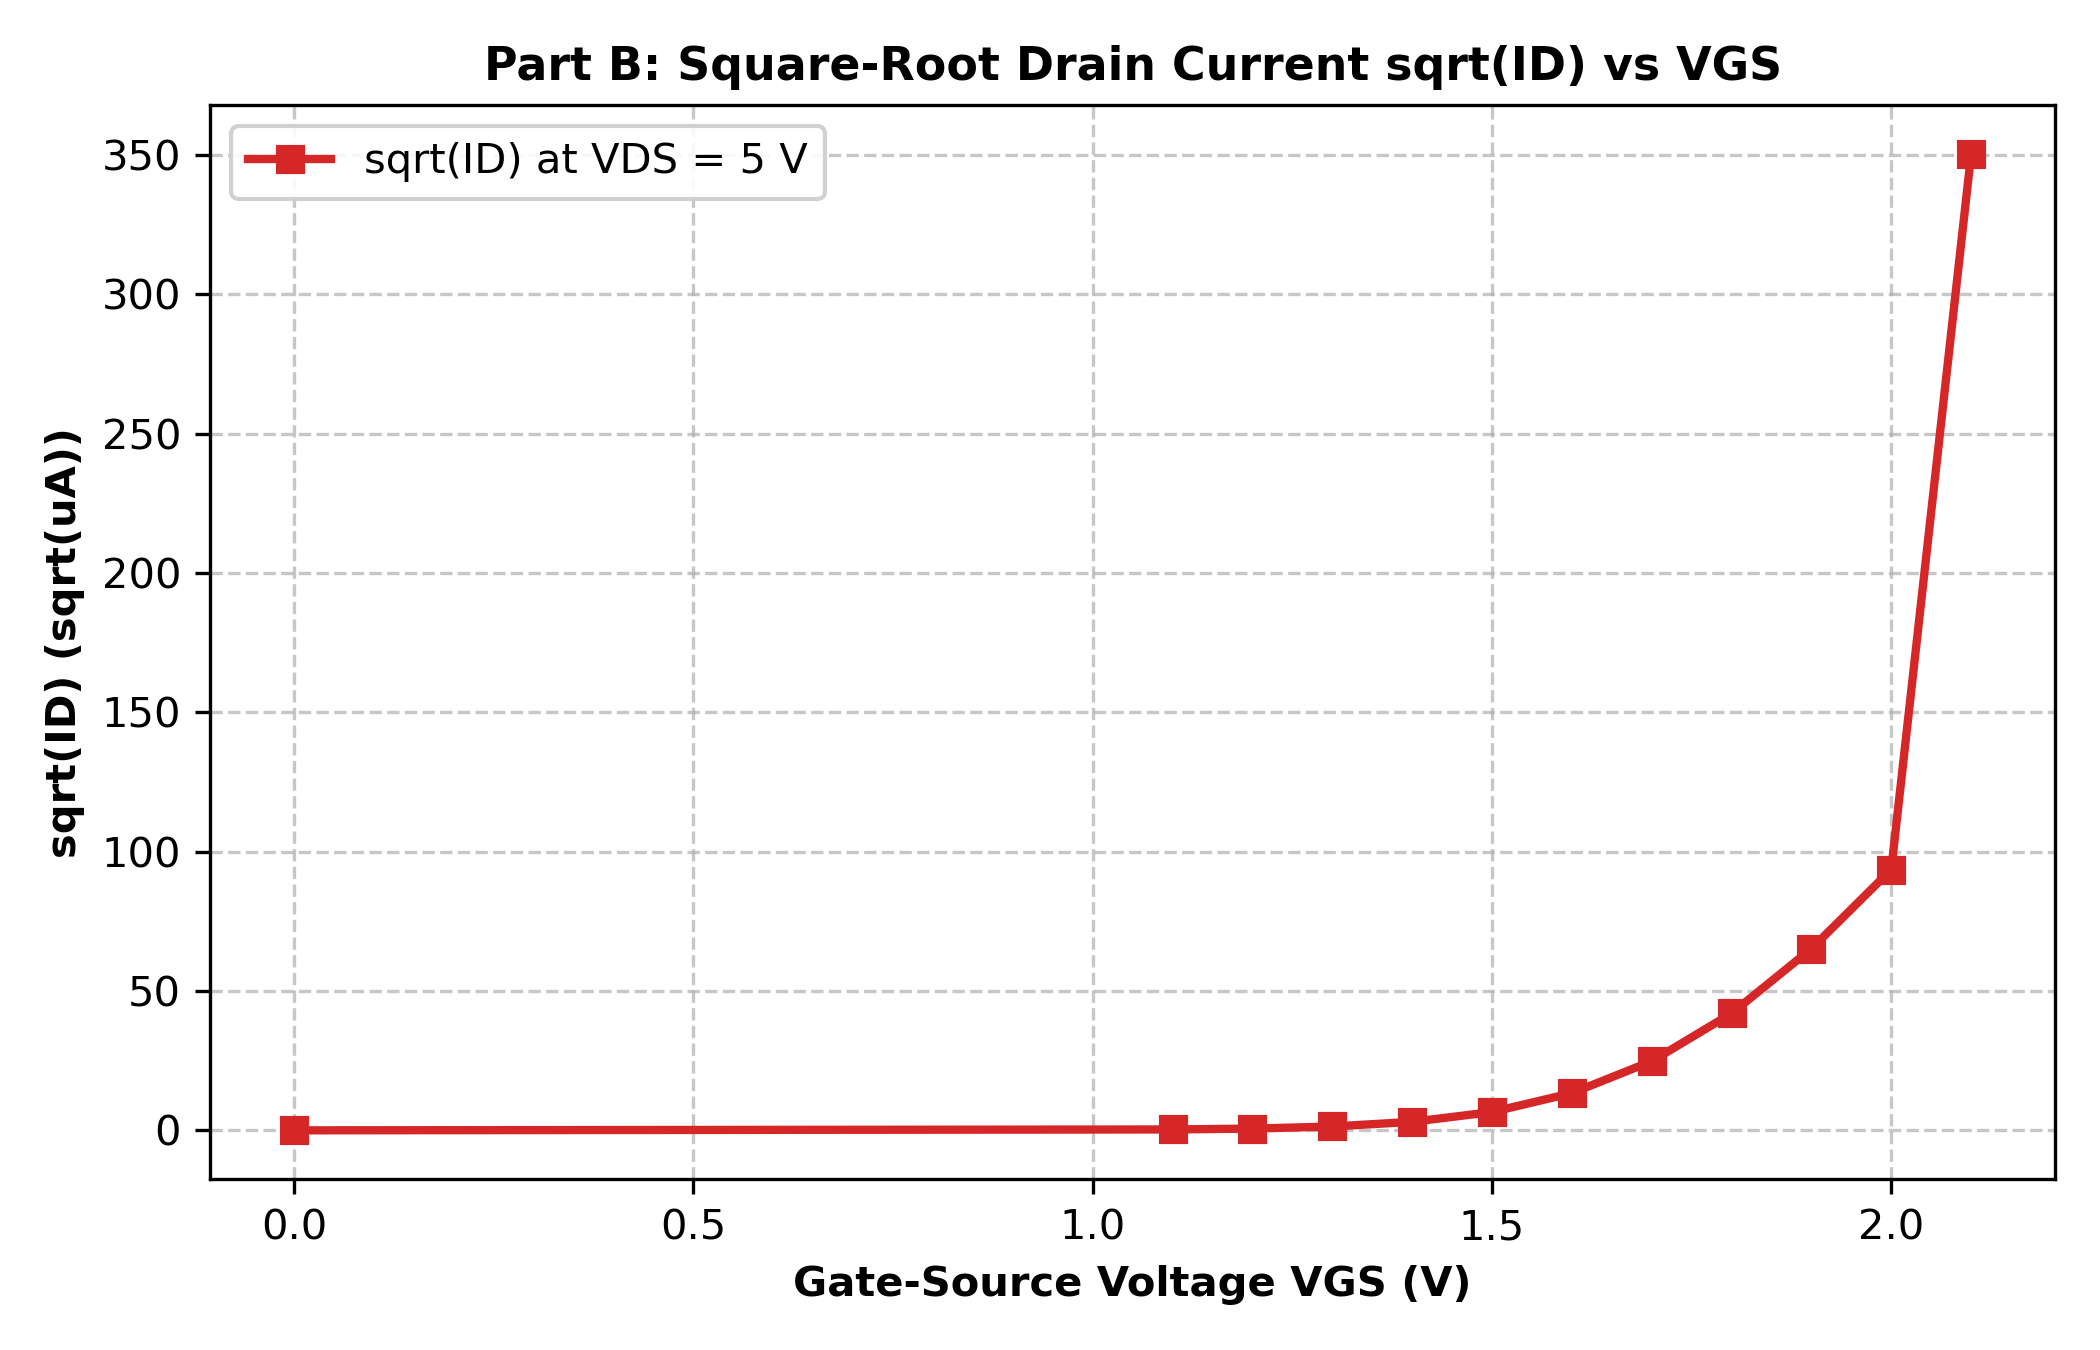
\includegraphics[width=\textwidth]{../PLOTS/PART_B_sqrt_ID.png}
        \caption{Square-Root Characteristic ($\sqrt{I_D}$ vs $V_{GS}$)}
    \end{subfigure}
    \caption{Combined Experimental Transfer Characteristics and $\sqrt{I_D}$ Extrapolation Plot.}
    \label{fig:part_b_combined_plots}
\end{figure}

\subsection{Calculations, Results, and Inferences (Part B)}
\begin{itemize}
    \item \textbf{Threshold Voltage ($V_T$) Determination:}
    \begin{itemize}
        \item From the dataset, conduction initiates at \textbf{$V_T \approx 1.10\text{ V}$}, where $I_D$ exceeds $0.1\ \mu\text{A}$.
        \item Extrapolating the linear portion of $\sqrt{I_D}$ vs $V_{GS}$ back to zero current confirms \textbf{$V_T = 1.10\text{ V}$}.
    \end{itemize}

    \item \textbf{Transconductance ($g_m$) Calculations ($V_{GS} = 1.6\text{ V}$ to $2.0\text{ V}$):}
    \begin{itemize}
        \item \textbf{At $V_{DS} = 5\text{ V}$:} $\Delta V_{GS} = 0.4\text{ V}$, $\Delta I_D = 8760.0 - 178.6 = 8581.4\ \mu\text{A} = 8.581\text{ mA}$.
        \[
        \mathbf{g_m(5\text{V}) = \frac{8.581\text{ mA}}{0.4\text{ V}} = 21.45\text{ mS}}
        \]
        \item \textbf{At $V_{DS} = 7\text{ V}$:} $\Delta V_{GS} = 0.4\text{ V}$, $\Delta I_D = 8770.0 - 178.6 = 8591.4\ \mu\text{A} = 8.591\text{ mA}$.
        \[
        \mathbf{g_m(7\text{V}) = \frac{8.591\text{ mA}}{0.4\text{ V}} = 21.48\text{ mS}}
        \]
        \item \textbf{At $V_{DS} = 9\text{ V}$:} $\Delta V_{GS} = 0.4\text{ V}$, $\Delta I_D = 8910.0 - 185.9 = 8724.1\ \mu\text{A} = 8.724\text{ mA}$.
        \[
        \mathbf{g_m(9\text{V}) = \frac{8.724\text{ mA}}{0.4\text{ V}} = 21.81\text{ mS}}
        \]
        \item \textbf{Average Measured Transconductance ($g_{m,\text{avg}}$):} \textbf{$g_m \approx 21.58\text{ mS}$}
    \end{itemize}

    \item \textbf{Amplification Factor ($\mu$) Calculation:}
    \begin{equation}
        \mathbf{\mu = g_m \cdot r_d = 21.58\text{ mS} \times 63.16\text{ k}\Omega = 1363.00}
    \end{equation}

    \item \textbf{Key Results \& Inferences (Part B):}
    \begin{itemize}
        \item \textbf{Square-Law Conduction:} For $V_{GS} > V_T = 1.10\text{ V}$, $I_D$ exhibits sharp quadratic growth, reaching several milliamperes as $V_{GS}$ approaches $2.0\text{ V}$.
        \item \textbf{Independence from $V_{DS}$ in Saturation:} The transfer curves for $V_{DS} = 5\text{ V}, 7\text{ V}, 9\text{ V}$ are virtually identical, demonstrating that the device is deeply in saturation and $I_D$ is purely controlled by $V_{GS}$.
    \end{itemize}
\end{itemize}

\clearpage

\section{Summary of Parameters and Final Conclusion}

\subsection{Summary of Extracted MOSFET Parameters}
\begin{table}[H]
\centering
\caption{Summary of Measured 2N7000 MOSFET Parameters}
\begin{tabular}{p{5.0cm} c c p{4.0cm}}
\toprule
\textbf{Parameter} & \textbf{Experimental Value} & \textbf{Datasheet Range} & \textbf{Remark} \\
\midrule
Threshold Voltage ($V_T$) & \textbf{1.10 V} & $0.8\text{--}3.0\text{ V}$ & \textbf{Within Limits} \\
Drain Resistance ($r_d$) & \textbf{63.16 k$\Omega$} & $10\text{--}100\text{ k}\Omega$ & \textbf{High Output Impedance} \\
Transconductance ($g_m$) & \textbf{21.58 mS} & $10\text{--}50\text{ mS}$ & \textbf{High Gain Capability} \\
Amplification Factor ($\mu$) & \textbf{1363.00} & $>1000$ & \textbf{Extremely High Voltage Gain} \\
\bottomrule
\end{tabular}
\end{table}

\section{Final Conclusion}
\begin{enumerate}
    \item The experimental analysis of the \textbf{2N7000 N-Channel Enhancement MOSFET} successfully verified the distinct triode ($V_{DS} < V_{GS} - V_T$) and saturation ($V_{DS} \geq V_{GS} - V_T$) operational regions.
    \item Part A output characteristics confirmed a high drain resistance of \textbf{$r_d \approx 63.16\text{ k}\Omega$}, reflecting flat saturation behavior in the active region.
    \item Part B transfer characteristics yielded a device threshold voltage of \textbf{$V_T = 1.10\text{ V}$} and a transconductance of \textbf{$g_m \approx 21.58\text{ mS}$}.
    \item The calculated amplification factor \textbf{$\mu = 1363.00$} highlights the superior voltage amplification capability and the voltage-controlled nature of MOSFETs compared to BJTs.
\end{enumerate}

\end{document}
